\setchapterstyle{kao}
\chapter{Search for sterile neutrino mixing}
\setchapterpreamble[u]{\margintoc}
\label{ch:measurement-sterile}

This analysis assumes the extended 3+1 neutrino PMNS framework, with the parameters to be constrained being the oscillation parameters $\theta_{24}$ and $\theta_{34}$.
The three-flavor atmospheric oscillation parameters and the CP-violating phase $\delta_{24}$ are treated as nuisance parameters.
The mass-splitting of the additional mass eigenstate is fixed at $\Delta m^2_{41}=1\;\mathrm{eV^2}$.
Because the oscillations at Earth-scale baselines occur on much smaller energy scales than can be resolved by DeepCore, the analysis effectively becomes indifferent to the magnitude of $\Delta m^2_{41}$ and constrains the values of $\theta_{24}$ and $\theta_{34}$ based on the \emph{averaged} oscillation effect.
As a consequence, the constraints calculated based on the assumption that $\Delta m^2_{41}=1\;\mathrm{eV^2}$ are still valid even if the true mass splitting is much larger.
This holds true up to mass splitting values of about $m^2_{41}\gtrapprox100\;\mathrm{eV^2}$, where the heavy mass eigenstate becomes so much slower than the light eigenstates that it would no longer interfere with them and decohere\cite{atmo_decoherence}.

\section{Atmospheric oscillations in the presence of an eV-scale sterile neutrino}

\subsection{The 3+1 model}
This analysis probes the "3+1" oscillation model, in which a fourth "sterile" (i.e., non-interacting) neutrino flavor eigenstate $\nu_s$ and mass eigenstate $\nu_4$ with mass splitting $\Delta m^2_{41}$ is added to the standard three-flavor model.
The PNMS mixing matrix is extended by a fourth row and column, which is parametrized with additional mixing angles $\theta_{14}$, $\theta_{24}$, $\theta_{34}$ and CP violating phases $\delta_{14}$ and $\delta_{24}$ as
\begin{align*}
    U_{3+1} =&\begin{pmatrix}
    U_{e1}    & U_{e2}    & U_{e3}   &U_{e4}    \\
    U_{\mu1}  & U_{\mu2}  & U_{\mu3} &U_{\mu4}  \\
    U_{\tau1} & U_{\tau2} & U_{\tau3}&U_{\tau4} \\
    U_{s1} & U_{s2} & U_{s3}&U_{s4} \\
    \end{pmatrix}\\
    =&
    R_{34}(\theta_{34})
    \tilde{R}_{24}(\theta_{24}, \delta_{24})
    \tilde{R}_{14}(\theta_{14}, \delta_{14})
    R_{23}(\theta_{23})
    \tilde{R}_{13}(\theta_{13}, \delta_{13})
    R_{12}({\theta_{12})}\;,
\end{align*}
where $R_{kl}$ are rotation matrices.
The goal of this analysis is to constrain the matrix elements $U_{\mu4}$ and $U_{\tau4}$ with magnitude $|U_{\mu4}|^2=\sin^2(\theta_{24})$ and  $|U_{\tau4}|^2=\sin^2(\theta_{34})\cos^2\theta_{24}$, respectively, via the measurement of $\nu_\mu$ disappearance.

In the presence of an eV-scale sterile neutrino, the standard three-flavor oscillation pattern as a function of neutrino energy and zenith angle is distorted and overlaid with a much faster secondary oscillation pattern.
\reffig{numu_survival_1eV2_full_range} shows the muon-neutrino survival probability in the presence of a fourth mass eigenstate with $\Delta m^2_{41}=1\;\mathrm{eV^2}$ and $\theta_{24}=15^\circ$ as a function of the energy and cosine of the zenith angle, where $\cos(\theta_z)=-1$ indicates that the neutrino is coming directly from below and $\cos(\theta_z)=1$ directly from above.
For up-going neutrinos, the oscillation pattern induced by $\Delta m^2_{41}$ is only resolved at energies of $>\mathcal{O}(1\;\mathrm{TeV})$.
Below $\sim$200~GeV, the oscillation length reaches values of as low as $\mathcal{O}(\mathrm{km})$, which makes them unresolvable below the horizon where baselines are of $\mathcal{O}(10000\;\mathrm{km})$.

\subsection{Neutrino production height effects}
Above the horizon, the distance from the upper layers of the atmosphere where the neutrinos are produced to the detector is small enough to create a distinct oscillation pattern for a fixed production height, as can be seen in the left panel of \reffig{numu_survival_1eV2_full_range}.
Because neutrino production heights vary over a range of tens of kilometers, it is necessary to average the oscillation probability over production heights to obtain a more realistic expectation.
This is done analytically in \texttt{nuSQuIDS}\cite{squids, nusquids} by calculating the averaged vacuum oscillation probability over a uniform distribution.
The right panel of \reffig{numu_survival_1eV2_full_range} shows the oscillation probability with production heights averaged between 10~km and 30~km.
The oscillation pattern above the horizon is no longer clearly resolvable, but an average disappearance effect for neutrino energies below 20~GeV remains.
The uniform distribution that is assumed to calculate the averaged oscillation probabilities is of course not entirely realistic.
For this reason, only events that arrive at most slightly above the horizon ($\cos(\theta_z)<0.1$) are included in this analysis.

\begin{figure}
    \centering
    \tikzsetnextfilename{numu_surv_compare_height_avg}%
\begin{tikzpicture}

\definecolor{darkgray176}{RGB}{176,176,176}

\begin{groupplot}[
    group style={
        group size=2 by 1,
        ylabels at=edge left,
        yticklabels at=edge left,
        horizontal sep=0.5 cm
    },
    log basis x={10},
    tick align=outside,
    tick pos=left,
    xlabel={energy (GeV)},
    xmin=2, xmax=5000,
    xmode=log,
    xtick style={color=black},
    y grid style={darkgray176},
    ylabel={\(\displaystyle \cos(\theta_{\mathrm{z}})\)},
    ymin=-1, ymax=1,
    ytick style={color=black},
    width=0.55\textwidth
]
\nextgroupplot[
    colorbar horizontal,
    colorbar style={
        xlabel={$P(\nu_\mu\rightarrow\nu_\mu)$},
        width=2*\pgfkeysvalueof{/pgfplots/parent axis width} + \pgfkeysvalueof{/pgfplots/group/horizontal sep},
        height=0.35cm,
        anchor=south west,
        at={(0, 1.05)},
        xticklabel pos=upper,
        tick pos=upper
    },
    colormap={mymap}{[1pt]
      rgb(0pt)=(0.368627450980392,0.309803921568627,0.635294117647059);
      rgb(1pt)=(0.196078431372549,0.533333333333333,0.741176470588235);
      rgb(2pt)=(0.4,0.76078431372549,0.647058823529412);
      rgb(3pt)=(0.670588235294118,0.866666666666667,0.643137254901961);
      rgb(4pt)=(0.901960784313726,0.96078431372549,0.596078431372549);
      rgb(5pt)=(1,1,0.749019607843137);
      rgb(6pt)=(0.996078431372549,0.87843137254902,0.545098039215686);
      rgb(7pt)=(0.992156862745098,0.682352941176471,0.380392156862745);
      rgb(8pt)=(0.956862745098039,0.427450980392157,0.262745098039216);
      rgb(9pt)=(0.835294117647059,0.243137254901961,0.309803921568627);
      rgb(10pt)=(0.619607843137255,0.00392156862745098,0.258823529411765)
    },
    point meta max=1,
    point meta min=0,
]
\addplot graphics [includegraphics cmd=\pgfimage,xmin=1, xmax=10000, ymin=-1, ymax=1] {figures/measurement/sterile_analysis/oscillation_signal/numu_surv_sterile_1eV_th24_15deg_noheightfilter-000.png};

\node[plot annotation, anchor=north east] at (axis description cs:0.99, 0.99) {$h_\mathrm{prod}=20\;\mathrm{km}$};

\nextgroupplot
\addplot graphics [includegraphics cmd=\pgfimage,xmin=1, xmax=10000, ymin=-1, ymax=1] {figures/measurement/sterile_analysis/oscillation_signal/numu_surv_sterile_1eV_th24_15deg_withheightfilter-000.png};

\node[plot annotation, anchor=north east] at (axis description cs:0.99, 0.99) {$10\;\mathrm{km} < h_\mathrm{prod} < 30\;\mathrm{km}$};

\end{groupplot}

\end{tikzpicture}

    \caption{Muon neutrino survival probability in the presence of a fourth mass eigenstate with $\Delta m^2_{41}=1\;\mathrm{eV^2}$ and $\theta_{24}=15^\circ$ with a fixed production height of 20~km (left) and with production heights averaged between 10~km and 30~km (right).\label{fig:numu_survival_1eV2_full_range}}
\end{figure}
%\begin{figure*}
%    \centering
%    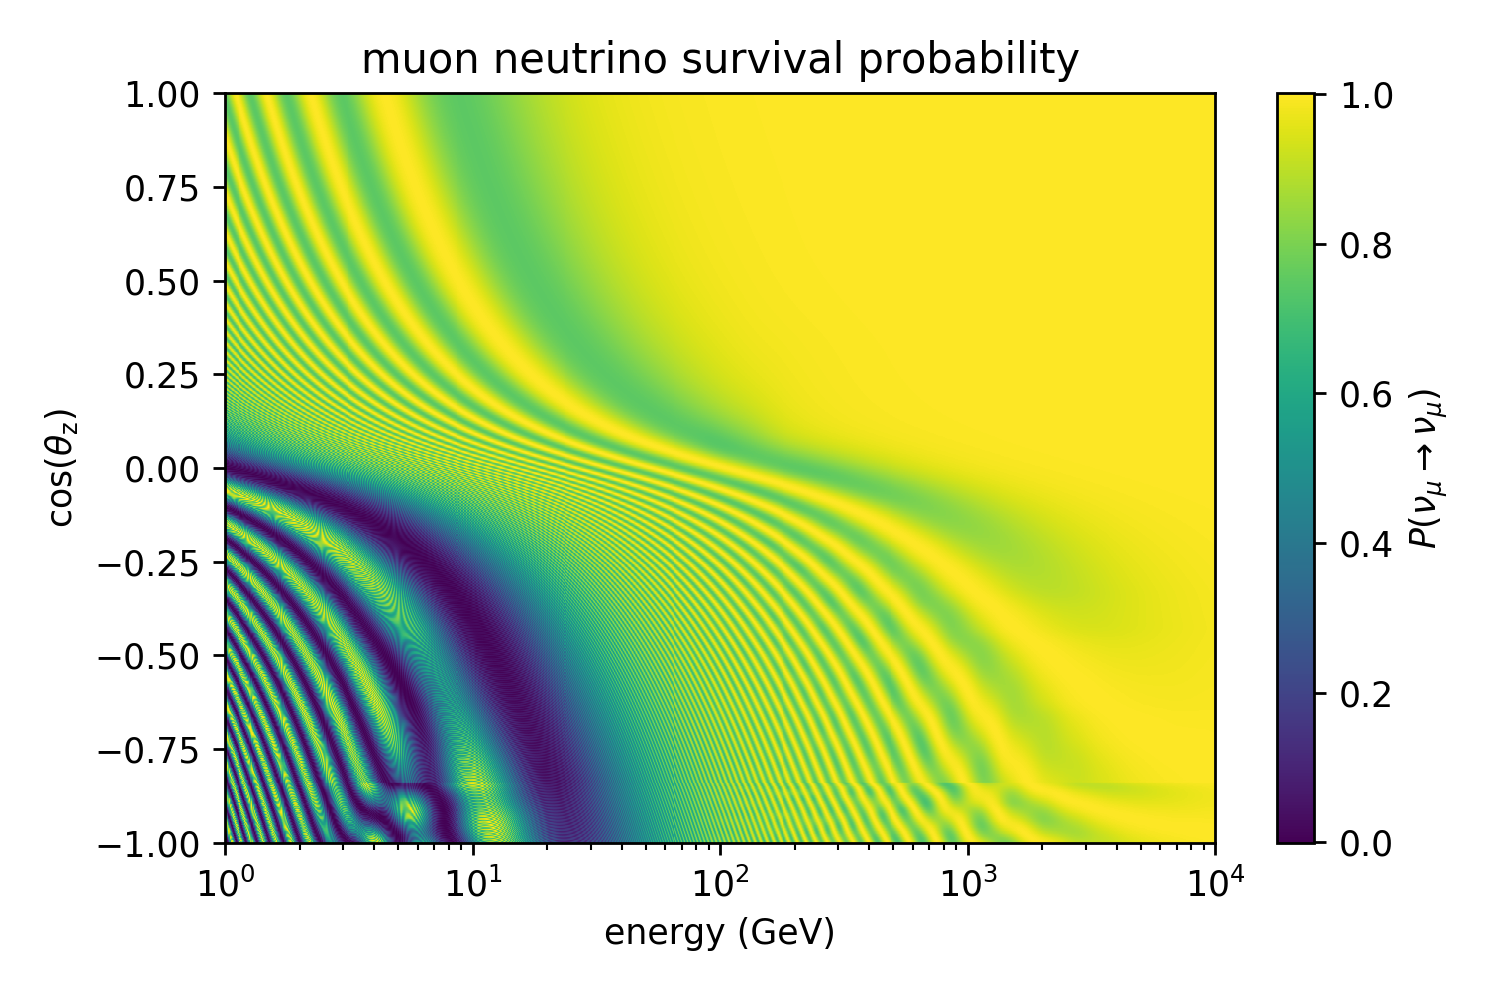
\includegraphics[width=0.45\linewidth]{figures/measurement/sterile_analysis/physics/dm41_0.5eV2_th24_15deg_no_filter.png}
%    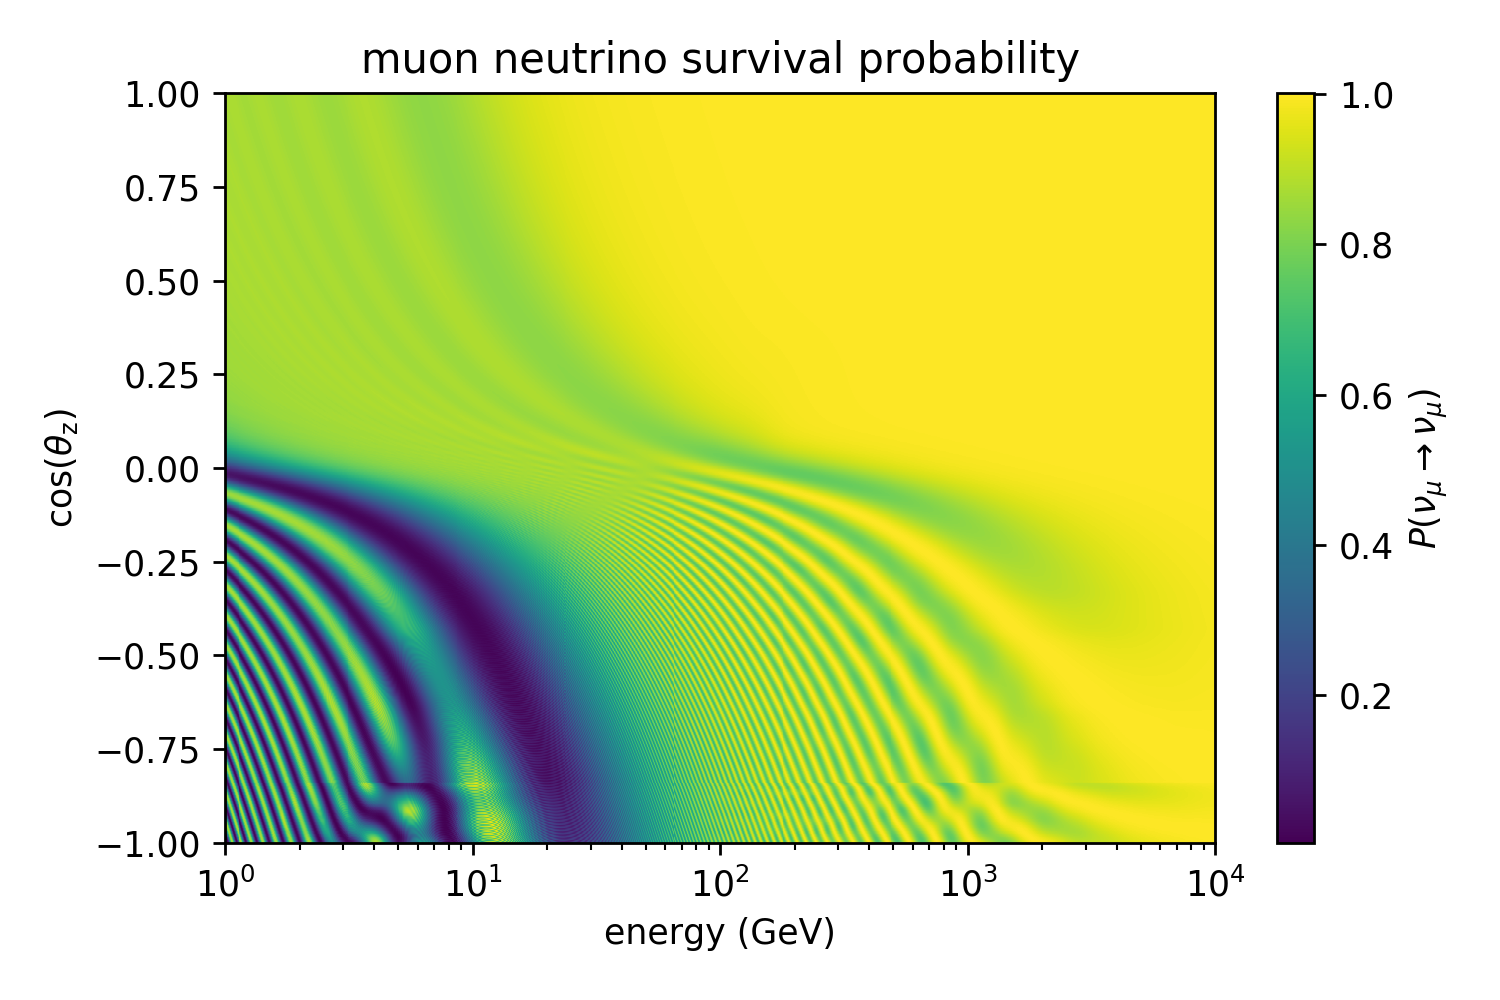
\includegraphics[width=0.45\linewidth]{figures/measurement/sterile_analysis/physics/dm41_0.5eV2_th24_15deg_avg_height_10-30km.png}
%    \caption{Muon neutrino survival probability in the presence of a fourth mass eigenstate with $\Delta m^2_{41}=0.5\;\mathrm{eV^2}$ and $\theta_{24}=15^\circ$ with a fixed production height of 20~km (left) and with production heights averaged between 10~km and 30~km (right).}
%    \label{fig:numu_survival_0.5eV2_full_range}
%\end{figure*}

\subsection{Oscillation signal for large mass splittings}
In the mass-splitting range where $\Delta m_{41}\approx\mathcal{O}(1\,\mathrm{eV^2})$ and in the energy range of the event sample ($<150\;\mathrm{GeV}$), the presence of a sterile neutrino produces rapid oscillations overlaid on the standard three-flavor oscillation pattern as well as distortions to that pattern itself as shown in \reffig{numu_survival_1eV2_analysis_binning_range} for a mixing angle of $\theta_{24}=15^\circ$.
The oscillation frequency in energy is too large to be resolved by DeepCore, but the average effect still allows us to constrain the magnitudes of $U_{\mu4}$ and $U_{\tau4}$.
The precise value of $\Delta m^2_{41}$ has very little influence on the average amplitude of the oscillations and therefore cannot be recovered in this mass splitting regime.
The oscillation averages stay approximately constant up to mass splitting values of well above $100\;\mathrm{eV^2}$ where decoherence effects begin to play a role\cite{atmo_decoherence}.
\begin{figure*}
    \centering
    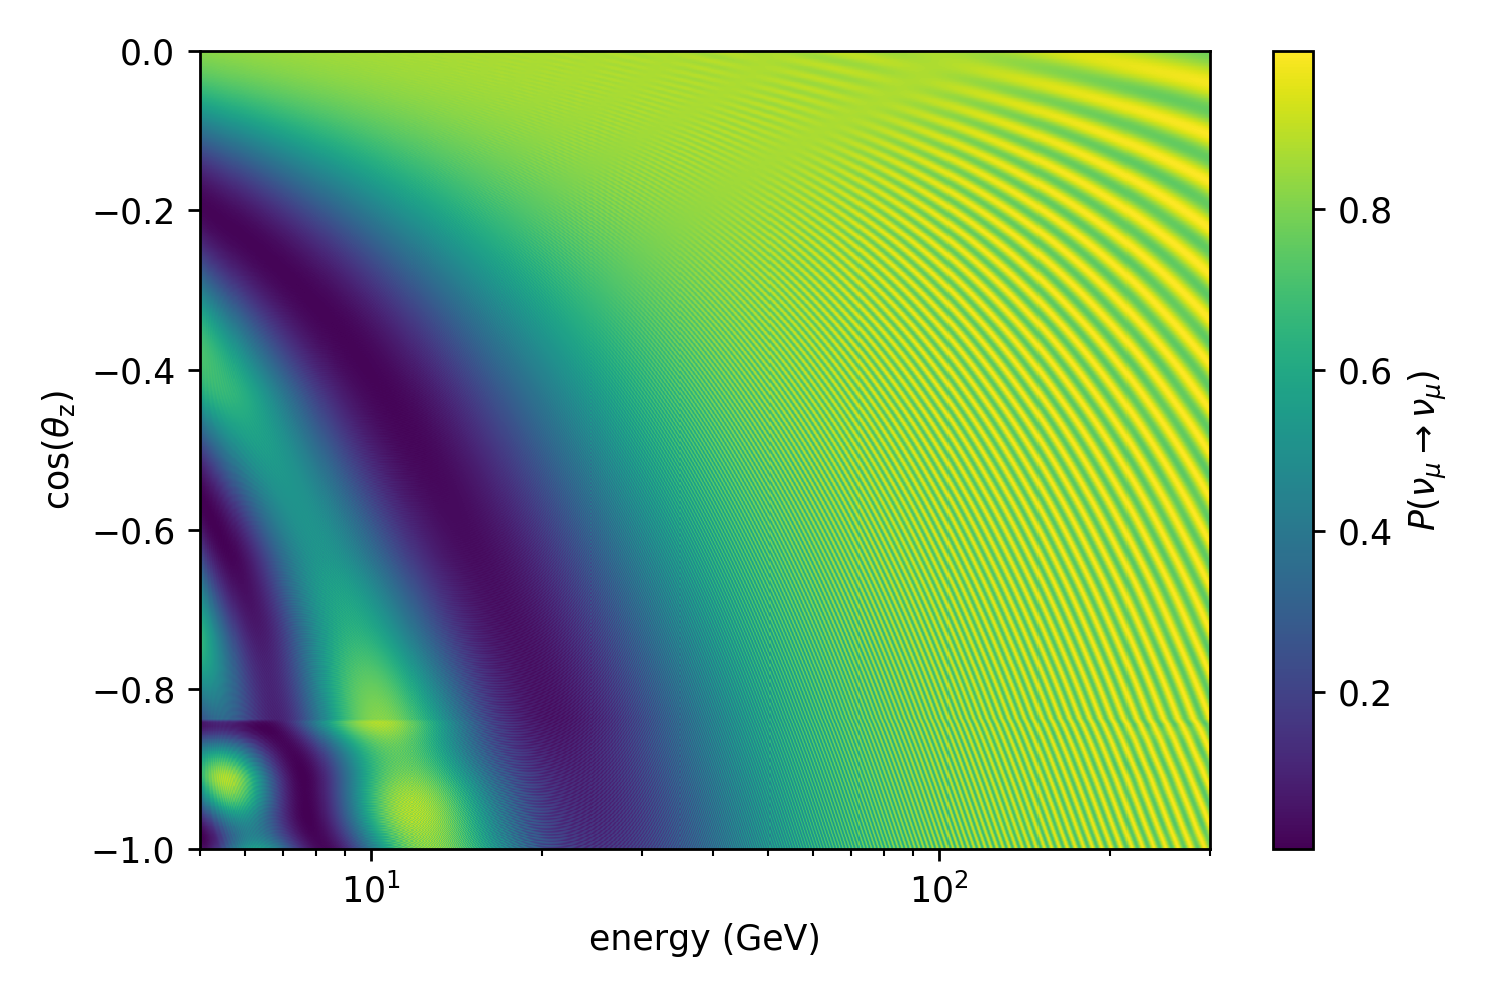
\includegraphics[width=0.45\linewidth]{figures/measurement/sterile_analysis/physics/dm41_1.0eV2_th24_15deg_avg_height_10-30km_ana_binning_range.png}
    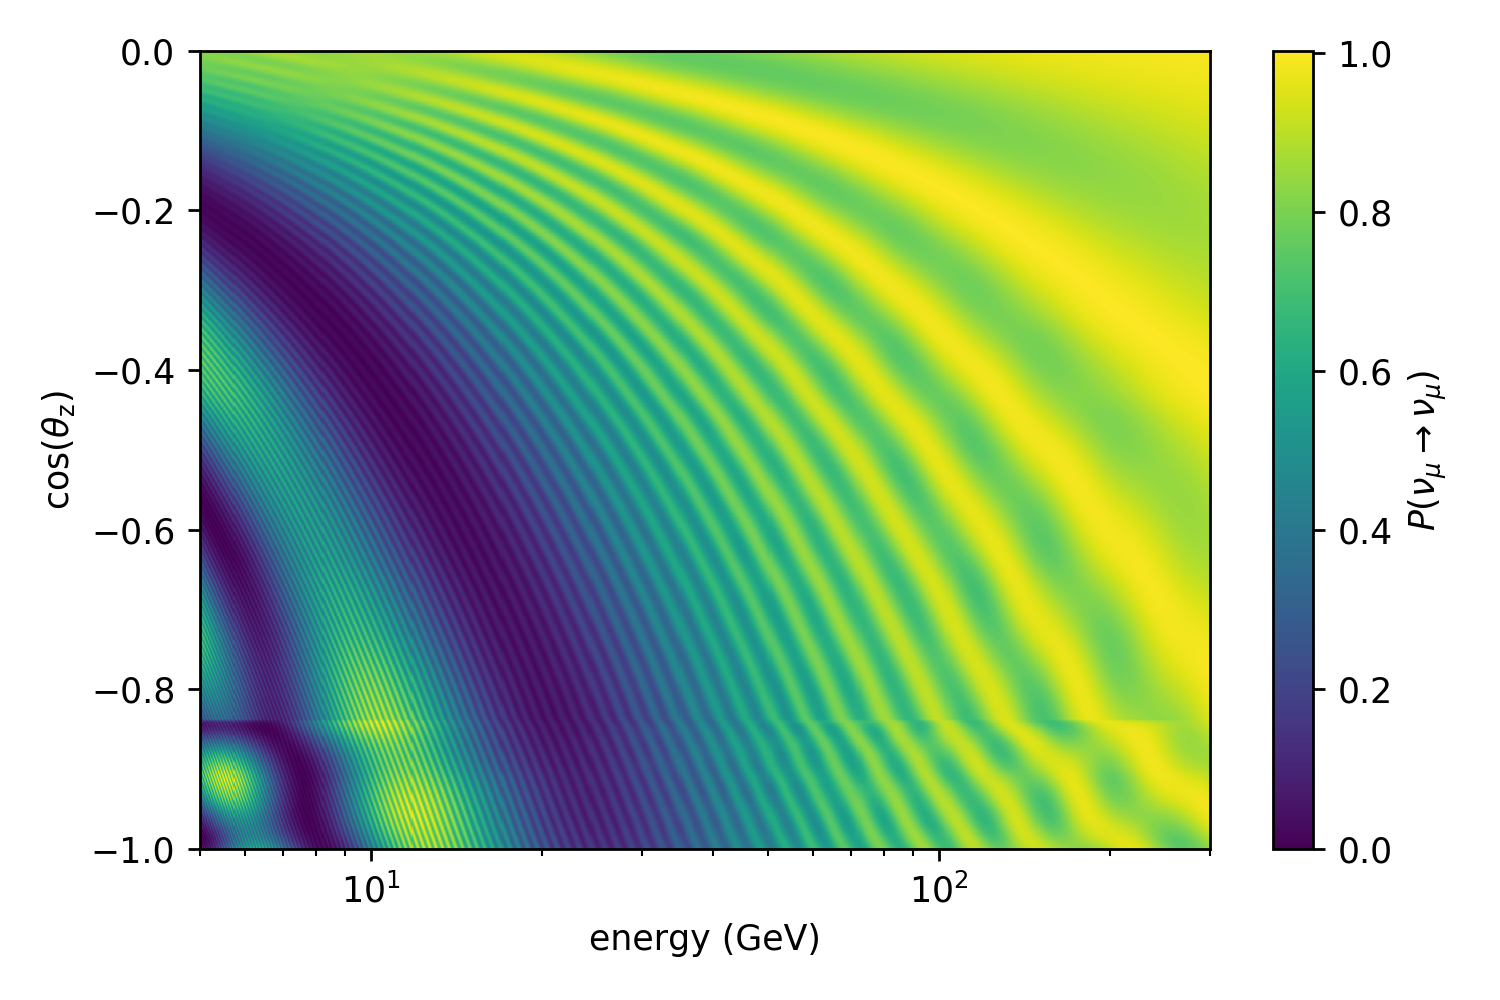
\includegraphics[width=0.45\linewidth]{figures/measurement/sterile_analysis/physics/dm41_0.1eV2_th24_15deg_avg_height_10-30km_ana_binning_range.png}
    \caption{$\nu_{\mu}$ survival probability at $\Delta m^2_{41}=1\;\mathrm{eV^2}$ (left) and at $\Delta m^2_{41}=0.1\;\mathrm{eV^2}$ (right). The mixing angle is $\theta_{24}=15^\circ$ in both cases}
    \label{fig:numu_survival_1eV2_analysis_binning_range}
\end{figure*}

\subsection{Oscillation signal for small mass splittings}
For mass-splitting values of $\Delta m^2_{41}$ well below $1\;\mathrm{eV^2}$, the oscillation pattern is no longer completely averaged out.
The right panel of \reffig{numu_survival_1eV2_analysis_binning_range} shows the muon-neutrino survival probability in the presence of a sterile neutrino state with mass splitting $\Delta m^2_{41}=0.1\;\mathrm{eV^2}$ and mixing angle $\theta_{24}=15^\circ$.
The highest oscillation minimum in energy and cosine of the zenith angle (upper right corner of the figure) is large enough to be resolvable with DeepCore.
This makes it possible in principle to produce constraints of the mixing matrix elements as a function of the mass-splitting $\Delta m^2_{41}$, although this is beyond the scope of the analysis presented in this thesis.
% \begin{figure}
%     \centering
%     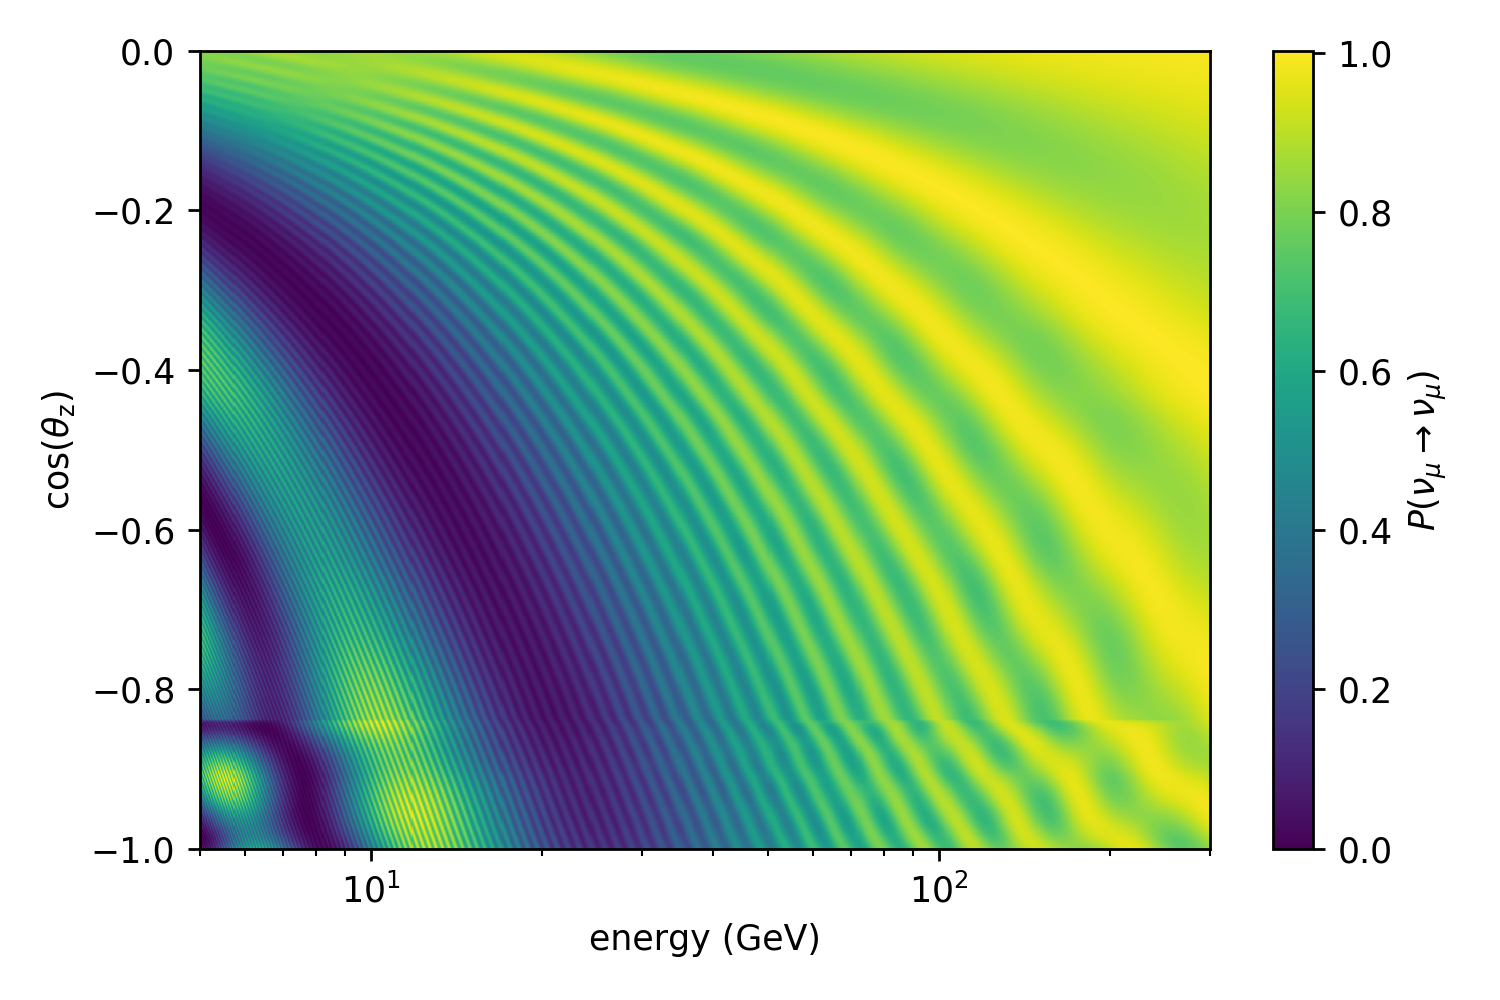
\includegraphics[width=0.8\textwidth]{figures/measurement/sterile_analysis/physics/dm41_0.1eV2_th24_15deg_avg_height_10-30km_ana_binning_range.png}
%     \caption{$\nu_{\mu}$ survival probability at $\Delta m^2_{41}=0.1\;\mathrm{eV^2}$ and $\theta_{24}=15^\circ$}
%     \label{fig:numu_survival_0.1eV2_analysis_binning_range}
% \end{figure}

\section{Oscillation Probability Calculation with \textsc{nuSQuIDS}}
\label{sec:nusquids}

This analysis uses as customized version of the neutrino Simple Quantum Integro-Differential Solver (\textsc{nuSQuIDS})\cite{squids, nusquids} package to calculate oscillation probabilities.
The basic principle behind \textsc{nuSQuIDS} is to calculate the state transition probabilities in the Interaction (Dirac) Picture of quantum mechanics, where the Hamiltonian is divided into the time-independent vacuum oscillation part $H_0$ and the time-dependent interaction part $ H_1(t)$:
\begin{equation}
    H(t) = H_0 + H_1(t)
\end{equation}
In this picture, the operators evolve with $ H_0$ as
\begin{equation}
\bar{O}_I(t)=e^{iH_0t}O_Se^{-iH_0t}\,,
\end{equation}
while state densities evolve with the interaction Hamiltonian $ H_1(t)$
\begin{equation}
\partial_t\bar{\rho}_I(t)=-i[\bar{H}_{1, I}(t), \bar{\rho}_I(t)]\,.
\end{equation}

This state evolution is solved by numerical integration in \textsc{nuSQuIDS}, which is computationally expensive.
However, because fast oscillations within $ H_0$ only play a sub-leading role, this difficult calculation does not have to be performed at every point in the analysis space.
It is sufficient to calculate state densities at a selected set of points, referred to as \emph{nodes}, and to then interpolate the densities between them.
The fast oscillations between the \textsc{nuSQuIDS} nodes are recovered when the probabilities for each flavor, $i$, are projected out with the trace operation on the state density with the (time-evolved) projection operator for that state:
\begin{equation}
p_i(t)=\mathrm{Tr}(\underbrace{\bar{\Pi}^{(i)}(t)}_{\mathrm{proj.\,op.}}\bar{\rho}_I(t))
\end{equation}

\subsection{Node placement}
The nodes where the difficult state integration is calculated do not need to be spaced densely enough in the analysis space to resolve the fast oscillations due to sterile neutrinos, but they do need to resolve matter effects. The state densities change most rapidly (as function of energy) for neutrinos that traverse a lot of matter at low energies. Additionally, there is a sharp break at $\cos(\theta_{\mathrm{zenith}})=-0.84$ where neutrinos begin to pass through the core.
For this reason, the \textsc{nuSQuIDS} nodes are concentrated in three places:
\begin{itemize}
    \item the energy region between 2 GeV and 10 GeV
    \item within a small interval around $\cos(\theta_{\mathrm{zenith}})=-0.84$
    \item the region below $\cos(\theta_{\mathrm{zenith}})=-0.84$
\end{itemize}
\reffig{nusquids-nodes} shows the optimized placement of \textsc{nuSQuIDS} nodes as black dots.

\begin{figure}
    \centering
    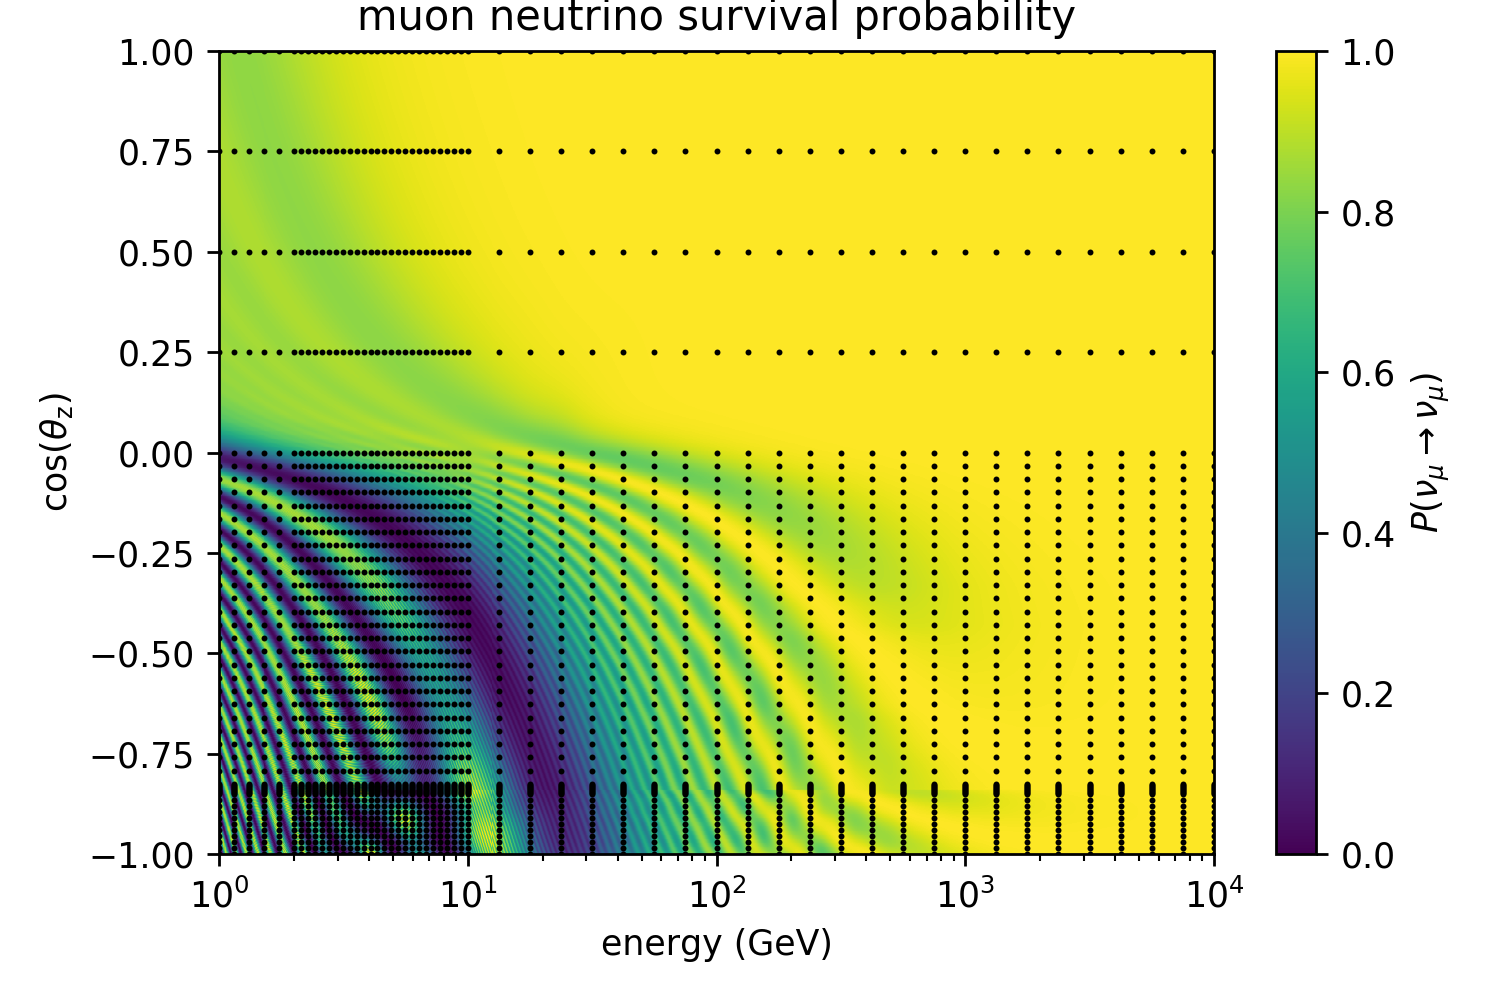
\includegraphics[width=0.7\textwidth]{figures/measurement/sterile_analysis/nusquids/0.1eV_sterile_only_height_avg_optim_nodes.png}
    \caption{Optimized placement of \textsc{nuSQuIDS} nodes (black dots) with extra dense node spacing in the three critical regions. The injected value for $\Delta m^2_{41}$ is $0.1\;\mathrm{eV^2}$.}
    \label{fig:nusquids-nodes}
\end{figure}

\subsection{Production height averaging}
At eV-scale mass splittings, oscillations are fast enough that significant oscillations occur even at 10-km-scale distances.
If the production height is assumed to be fixed at an exact position, a strong oscillation pattern appears above the horizon that could falsely produce a very high sensitivity in the analysis, driven entirely by events above the horizon.
In reality, production heights can vary within the atmosphere, which smears out the oscillations.
For this analysis, an analytical averaging method was implemented in nuSQuIDS that assumes a uniform distribution of propagation distances between two points.
The start and end point depends on the zenith angle and corresponds to the intersection of the neutrino path with a height of 10 km and 30 km, respectively.

\subsection{Low-pass filtering}
\label{sec:low-pass-filtering}
The fast oscillations in the presence of sterile neutrinos are filtered with a low-pass filter during both state evolution and the calculation of probabilities.
This step dramatically increases the speed with which oscillation probabilities can be evaluated.

Vacuum oscillations enter the differential equation governing the state evolution via the time evolution of the interaction Hamiltonian $\bar{H}_{1, I}(t)$.
At low energies, they cause tiny but extremely fast oscillations of the time derivative that the numerical integrator has to keep track of by drastically reducing the step size, slowing down the calculation.
To mitigate this problem and increase performance, a low-pass filter is applied when calculating the RHS of the differential equation.

\begin{figure}
    \centering
    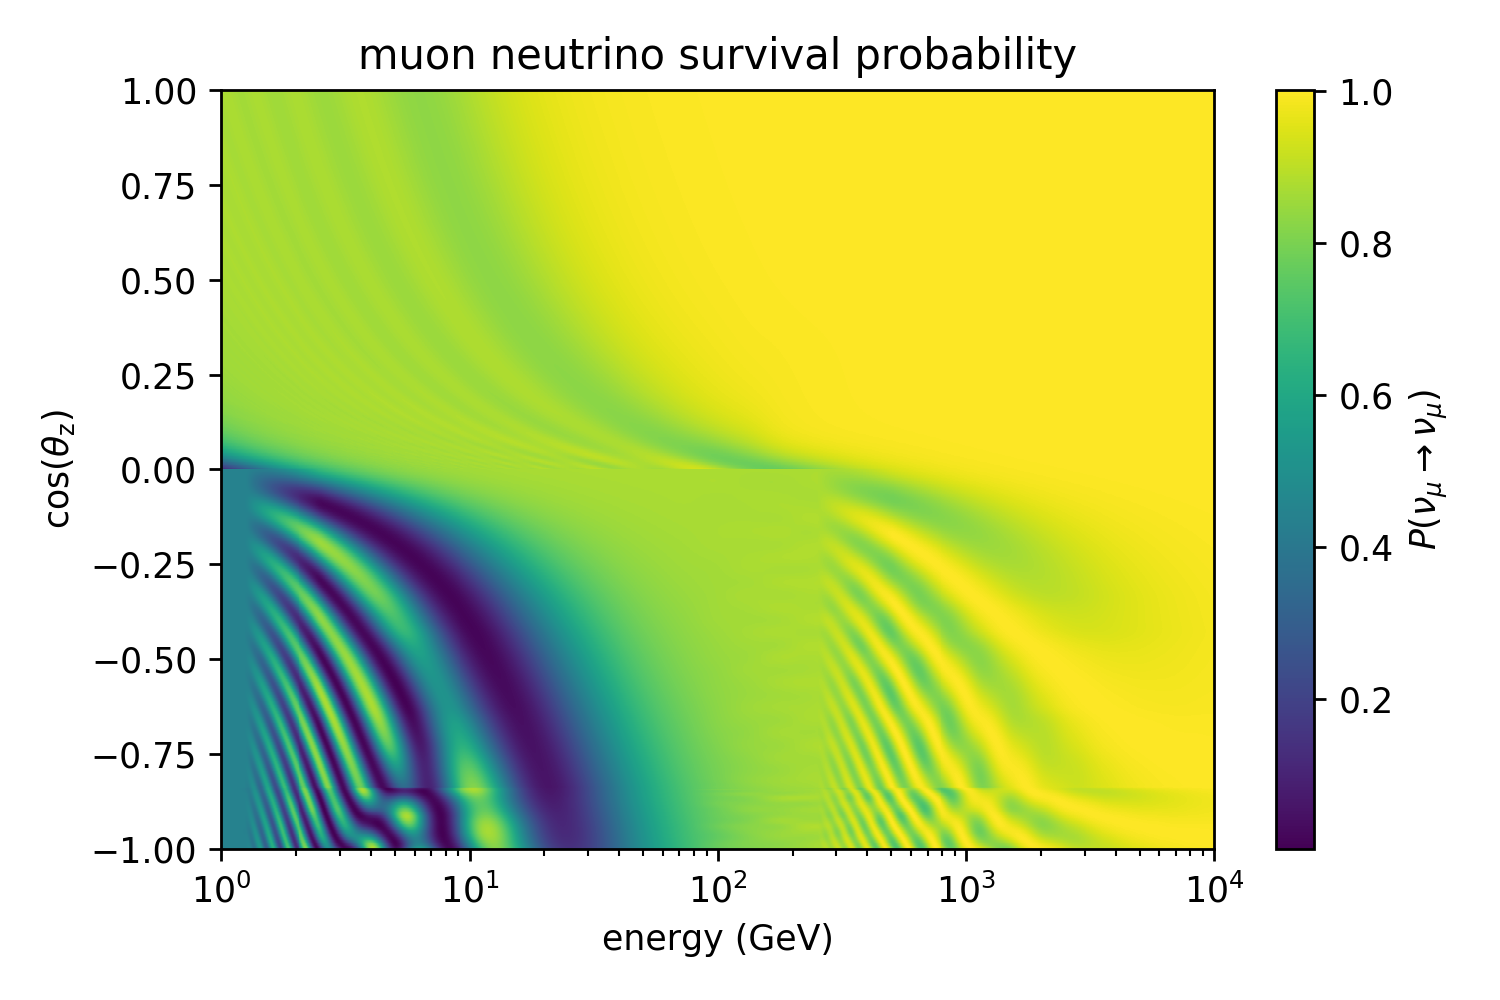
\includegraphics[width=0.7\textwidth]{figures/measurement/sterile_analysis/nusquids/Dm41_0.5eV2_th24_15deg_avg_height_10-30km_lp_belowhor.png}
    \caption{Muon neutrino survival probability in the presence of a sterile neutrino after application of both height averaging and low-pass filtering.}
    \label{fig:nusquids-low-pass-filtering}
\end{figure}

In the presence of sterile oscillations, transition probabilities usually have to be calculated for every single simulated event to average them out in the analysis binning.
Because the MC set has millions of events, doing this would be very expensive even when using nuSQuIDs' state interpolation feature.
In this analysis, a low-pass filter as a function of energy is applied when the transition probabilities are projected out from the state densities to average out very fast oscillations.
With this filtering, it is possible to calculate oscillation probabilities on a fine binning with ~20k bins.
One caveat is that this filtering is not appropriate to apply above the horizon because propagation distances there are short enough that oscillation probabilities don't average out completely.
Therefore, it is applied only below the horizon as shown in \reffig{nusquids-low-pass-filtering}.

\subsubsection{Test of Filter Performance}

To ensure that the chosen cut-off points of the low-pass filters do not introduce significant distortions to the oscillation signal, an inject/recover test is performed on a grid in $|U_{\mu 4}|$ and $|U_{\tau 4}|$ where pseudo-data is produced \emph{without} any low-pass filtering and fit back with the filtering enabled. For every grid point, a second fit is run where $\theta_{24}$ and $\theta_{34}$ are fixed to their true injected values. The p-value of the difference in the test statistic between these two fits, $\Delta \chi^2_{\mathrm{mod}}$, can be interpreted as the significance with which the true value of the mixing angles would be rejected solely due to the mismodeling of the true oscillation probabilities. The results of the mixing parameters fit and the corresponding values of $\Delta \chi^2_{\mathrm{mod}}$ are shown in \reffig{asimov-test-sterile-ana}. Assuming that $\Delta \chi^2_{\mathrm{mod}}$ should follow a $\chi^2$ distribution with two degrees of freedom, the significance of the mis-modeling is very small.
The fit errors for small values of $|U_{\mu 4}|$ and $|U_{\tau 4}|$ are insignificant because the likelihood is very flat in this region of the parameter space.
There are a few points for which the fit did not converge to the true global optimum, as indicated by a negative value of $\Delta \chi^2_\mathrm{mod}$, but the likelihood difference from the injected true parameters is also very small in these cases.

\begin{figure*}
    \centering
    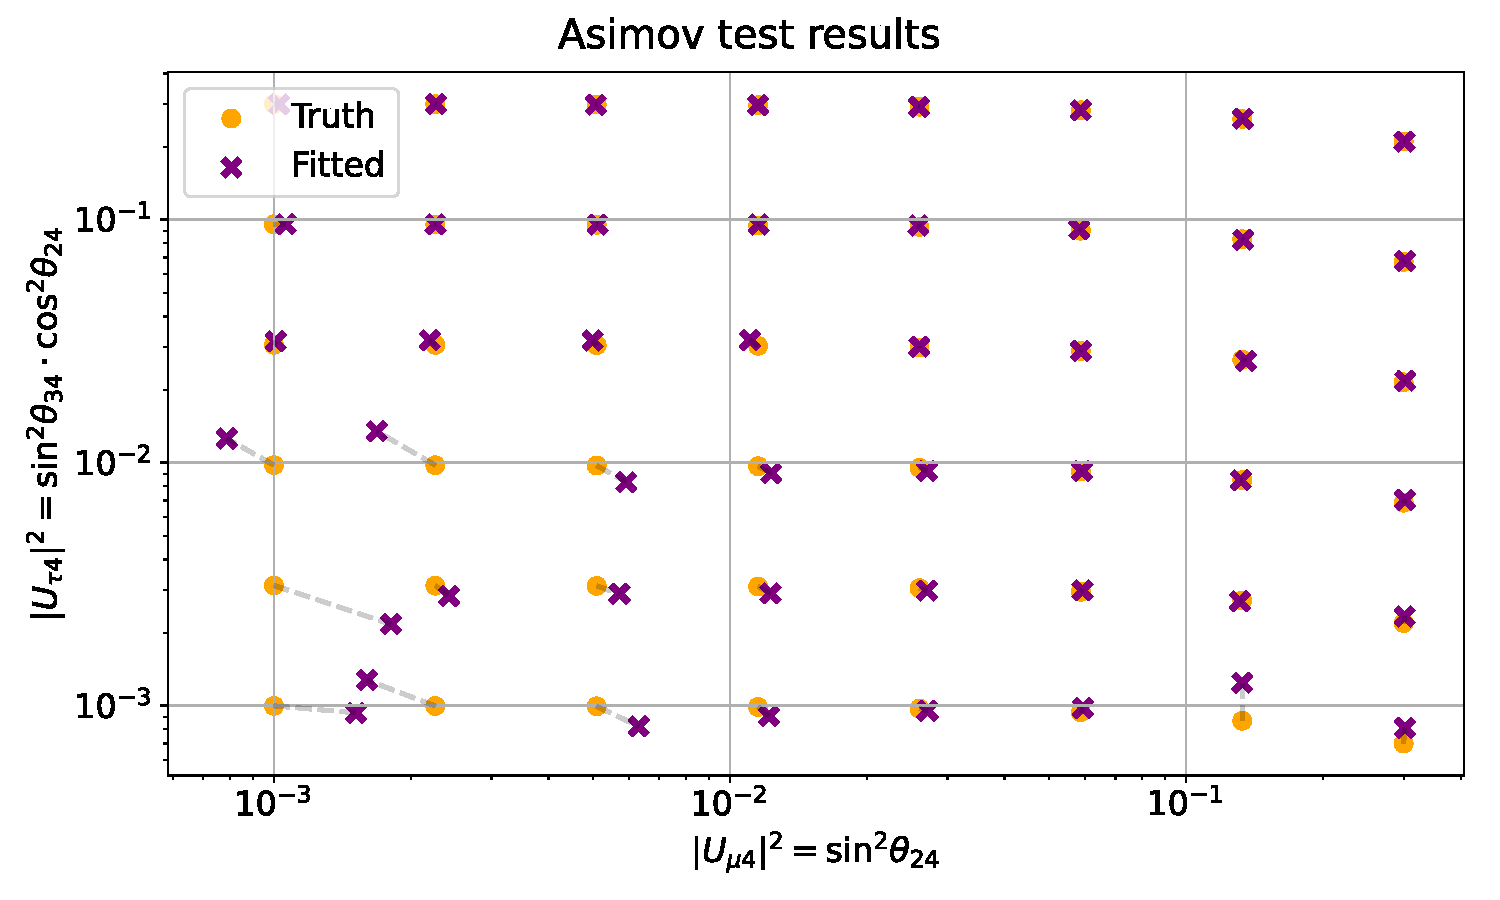
\includegraphics[width=0.49\linewidth]{figures/measurement/sterile_analysis/asimov_test/asimov_vs_v12_fit_err.pdf}
    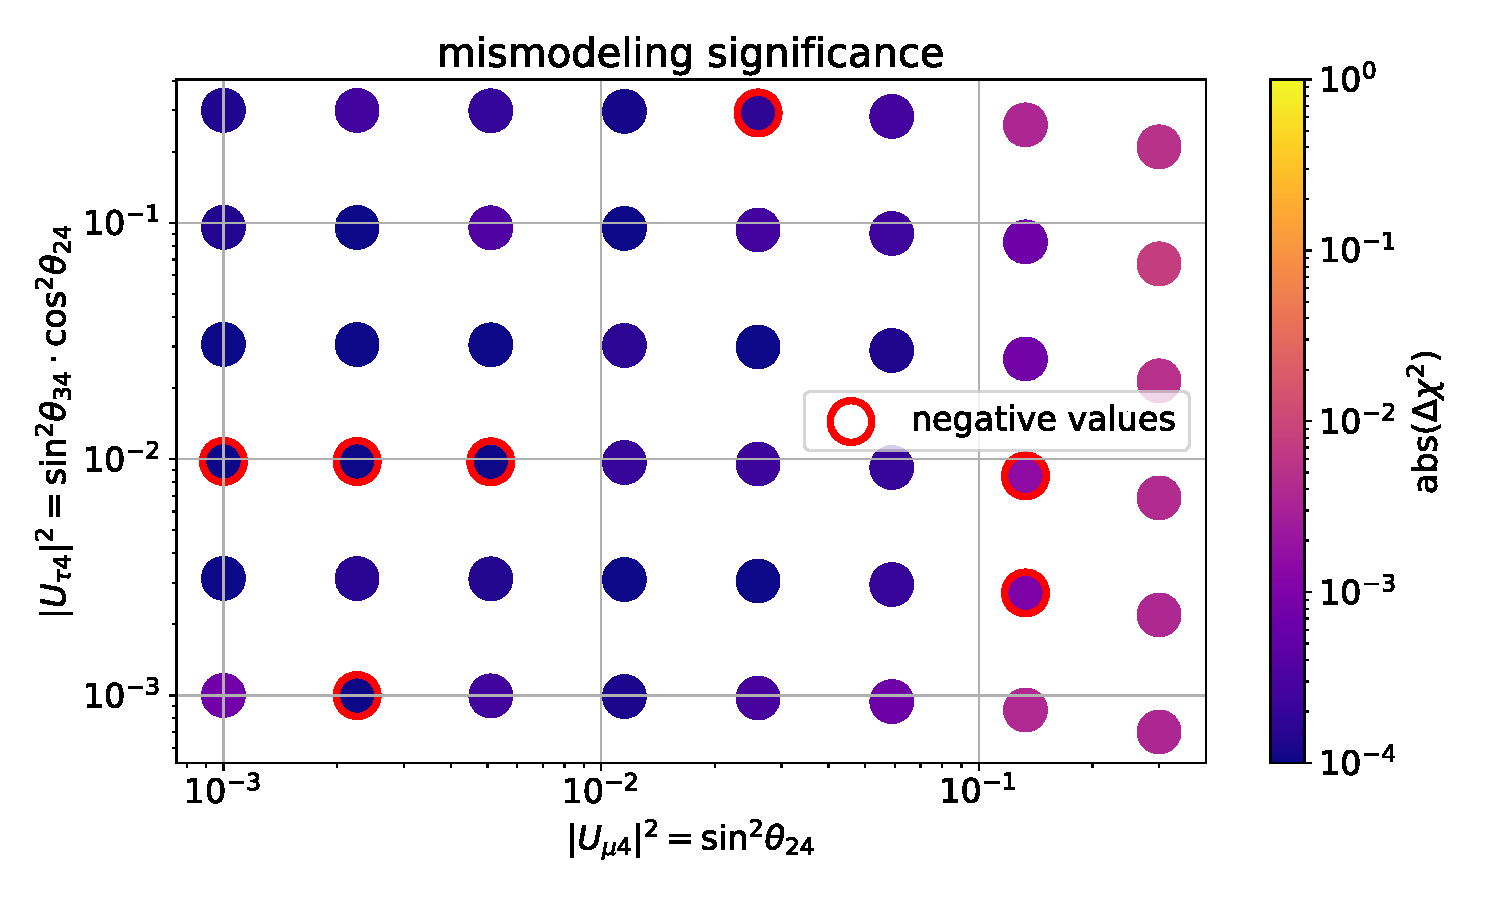
\includegraphics[width=0.49\linewidth]{figures/measurement/sterile_analysis/asimov_test/asimov_vs_v12_mismod.pdf}
    \caption{Results of the inject/recover test (left) and the corresponding mis-modeling values, $\Delta \chi^2_{\mathrm{mod}}$, attributable to low-pass filtering in \textsc{nuSQuIDS} (right). A negative value of $\Delta \chi^2_\mathrm{mod}$ indicates that the fit did not converge to the true global optimum.}
    \label{fig:asimov-test-sterile-ana}
\end{figure*}

\section{Nuisance oscillation parameters}
Besides the physics parameters $\theta_{24}$ and $\theta_{34}$ to be constrained by the analysis (at a fixed sterile mass splitting $\Delta m^2_{14}$), there are 4 additional mixing angles and 3 CP-violating phases in the 3+1 PNMS matrix as well as the mass splittings $\Delta m^2_{12}$ and $\Delta m^2_{13}$ that influence the oscillation probability. The solar and reactor angles $\theta_{12}$ and $\theta_{13}$ as well as the solar mass splitting $\Delta m^2_{12}$ are constrained by other experiments beyond the sensitivity of this analysis and are fixed at their current global best fit point\sidecite{nufit40}. The effect of the standard three-flavor CP violating phase $\delta_{\mathrm{CP}}=\delta_{13}$ is negligible and is fixed to zero.
The mixing angle $\theta_{14}$ and the phase $\delta_{14}$ are also fixed to zero, since recent reactor data constrains $|U_{e4}|^2 = \sin^2(\theta_{14})$ to $\mathcal{O}(10^{-3})$, which is well below the sensitivity of this analysis\sidecite{global_unitarity_Hu}.
The only nuisance parameters that remain free are the standard 3-flavor atmospheric oscillation parameters $\theta_{23}$ and $\Delta m^2_{13}$ as well as the sterile CP-violating phase $\delta_{24}$.
The effect of $\delta_{24}$ is to shift the oscillation pattern of muon neutrinos as shown in \reffig{sterile-cp-phase-effect}.
The effect runs in the opposite direction for \emph{anti}neutrinos.
Because neutrinos and antineutrinos are nearly indistinguishable in DeepCore, the combined effect of $\delta_{24}$ is a smearing of the oscillation minimum.
Additionally, the sign of $\cos(\delta_{24})$ is approximately degenerate with the neutrino mass hierarchy effect.
It is therefore expected that the analysis will produce very similar results for NO and IO when $\delta_{24}$ is free.
\reftab{oscillation-parameters} gives an overview over all oscillation parameters in the 3+1 model and their treatment in this analysis.
\begin{figure}
    \centering
    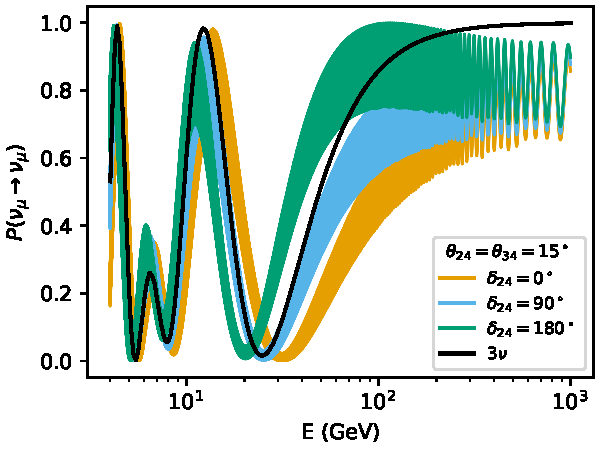
\includegraphics[width=0.8\textwidth]{figures/measurement/sterile_analysis/physics/oscillation_bands.pdf}
    \caption{Muon neutrino survival probability for a directly up-going neutrino as a function of energy in the presence of sterile neutrinos at different values of the sterile CP violating phase.}
    \label{fig:sterile-cp-phase-effect}
\end{figure}

\begin{table}
    \centering
    \begin{tabular}{@{}cccp{0.35 \linewidth}@{}}\toprule
        \textbf{parameter} & \textbf{nominal value} & \textbf{fixed?} & \textbf{comment} \\
        \midrule
        $\theta_{14}$ & $0^\circ$ & fixed &  Constr. by reactor data \\
        $\theta_{24}$ & -- & free & Physics parameter\\
        $\theta_{34}$ & -- & free & Physics parameter\\
        $\theta_{12}$ & $33.82^\circ$ & fixed & Constrained by reactor and solar data \\
        $\theta_{13}$ & $8.61^\circ$ & fixed & Constrained by reactor and accelerator data \\
        $\theta_{23}$ & $49.6^\circ$ & free & Atm. mixing angle \\
        $\delta_{13}$ & $0^\circ$ & fixed &  Negligible effect \\
        $\delta_{14}$ & $0^\circ$ & fixed &  No effect when $\theta_{14} = 0^\circ$ \\
        $\delta_{24}$ & -- & free & Smears osc. minimum \\
        $\Delta m^2_{21}$ & $7.39\times10^{-5}\;\mathrm{eV^2}$ & fixed & Constrained by reactor and solar data \\
        $\Delta m^2_{31}$ & $2.525\times10^{-3}\;\mathrm{eV^2}$ & free & Atm. mass splitting \\
        $\Delta m^2_{41}$ & $1\;\mathrm{eV^2}$ & fixed & Averaged out above $1\;\mathrm{eV^2}$ \\
        \bottomrule
    \end{tabular}
    \caption{Oscillation parameters of the 3+1 model and their treatment in this analysis.}
    \label{tab:oscillation-parameters}
\end{table}

\section{Statistical Analysis}

\subsection{Signal in Analysis Binning}
The change in bin counts with respect to the nominal expectation for different combinations of sterile mixing angles at $\Delta m^2_{41}=1\;\mathrm{eV^2}$ is shown in \reffig{oscillation-effects-ana-binning}.
Although a pull in only $\theta_{34}$ by $20^\circ$ has only a very small effect (see the middle panels of \reffig{oscillation-effects-ana-binning}), the combination of both angles can greatly amplify the signal.
The CP-violating phase $\delta_{24}$ only plays a role when both angles $\theta_{24}$ and $\theta_{34}$ are non-zero.
The sensitivity of this analysis to $\theta_{34}$ is entirely due to matter effects experienced by neutrinos passing through the dense core of the Earth.

\begin{figure}
    \centering
    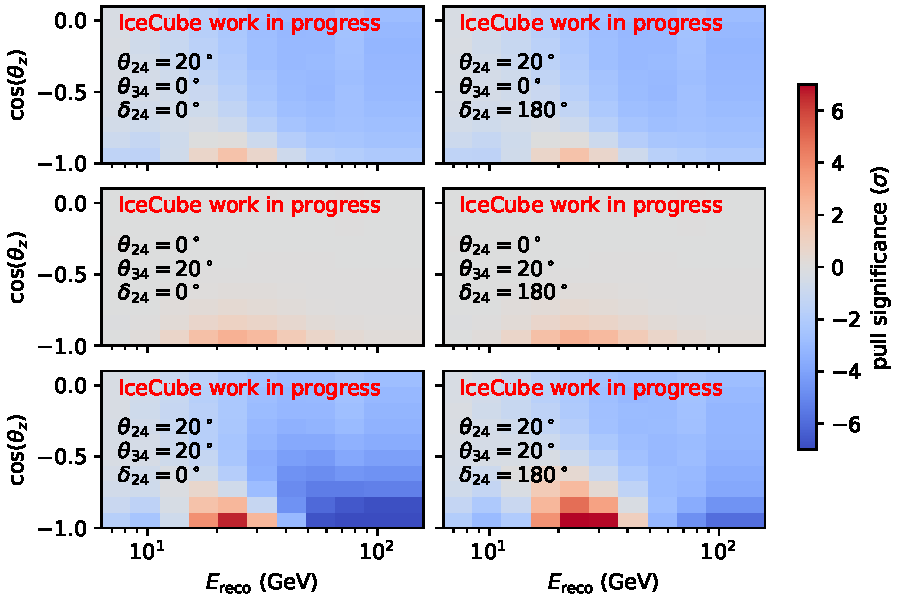
\includegraphics[width=0.95\textwidth]{figures/measurement/sterile_analysis/oscillation_signal/pull_theta_combinations_20deg_dcp24.pdf}
    \caption{Signal in the analysis binning produced by different combinations of $\theta_{24}$, $\theta_{34}$, and $\delta_{24}$ as a fraction of the Poisson error in each bin. The mass splitting of the sterile state is $\Delta m^2_{41}=1\;\mathrm{eV^2}$.}
    \label{fig:oscillation-effects-ana-binning}
\end{figure}

\subsection{Definition of test statistic}
\label{sec:test-statistic-sterile}

The histograms of the data and the expected values estimated by MC are compared using the same modified $\chi^2$ likelihood described in \refsec{test-statistic} that is also used for the three-flavor oscillation analysis.

\subsubsection{KDE error estimates}
To estimate the error on the KDE output, 20 bootstrap samples are drawn separately in each PID channel and the KDE is re-evaluated for each trial.
The expectation value and the standard deviation of the expectation in each bin of the histogram are the mean and standard deviation of these samples, respectively.
The samples are always produced with the same initial random seed to ensure that expectations and errors are reproducible.

\subsection{Modeling of detector response}
\label{sec:ultrasurfaces}

 As described in \refsec{hypersurfaces}, the gradients acquired by bin-wise linear regressions in the analysis histogram are only correct for the particular choice of the flux and oscillation parameters at which they have been fitted.
For the three-flavor analysis, this can be mitigated by a piece-wise interpolation of the gradients as a function of the mass splitting $\Delta m^2_{31}$, and the impact of other parameters is small enough that this one-dimensional interpolation is sufficient.
However, for the sterile analysis, several additional oscillation parameters have the potential to substantially change the shape of the oscillation pattern and therefore change the detector response in each bin.
The grid required to apply the interpolation to all potentially relevant parameters would have to have at least five dimensions and the RAM requirement to hold all those parameters would have been prohibitive.
It was therefore deemed necessary to develop an entirely new method for the treatment of detector systematic uncertainties that completely decouples the detector response from flux and oscillation weights, as described in this section.

The goal of this treatment of detector systematic effects is to find reweighting factors for every event in the nominal MC set that correspond to how much more or less likely that particular event would be if the detector properties were different.
These reweighting factors should be independent from any other event weights, especially flux and oscillation weights.
To get an intuition, one may look at an event in which the reconstructed energy is larger than the true energy.
In the case where the DOM efficiency is higher than nominal, the detector observes more light than is expected from the baseline simulation, and it becomes more likely that such an event occurs and it should therefore get more weight.
On the other hand, if the DOM efficiency is smaller, the reconstructed energy will, on average, be biased downwards.
This makes an event with an overestimated energy less likely and it should therefore get a smaller weight.
This relationship will not change depending on the initial flux of the primary neutrino or oscillation effects because the detector reacts only to the final state.

Using the discrete MC sets with different variations of detector parameters, one needs to find the re-weighting factors, $R_{ik}$, for each event in the nominal MC set, $i$, such that re-weighting every event by its weighting factor produces the same distribution in energy, zenith angle and PID as the off-nominal MC set, $k$.
If the true distributions of event parameters in each MC set was known, this weighting factor could be calculated as the ratio
\begin{equation}
    R_{ik} = \frac{P(X_i|\theta_k)}{P(X_i|\theta_{\rm nominal})} \frac{P(\theta_k)}{P(\theta_{\rm nominal})}\;, \label{eq:ratio-likelihood}
\end{equation}
where $\theta_k$ are the detector parameters of the off-nominal MC set, $k$.
The vector $X_i$ contains the true and reconstructed values for energy and zenith angle, as well as the PID of the event.
 The probability distribution $P(X_i|\theta_k)$ is the distribution of the event parameters in MC set $k$, and $\theta_{\rm nominal}$ contains the values of the detector parameters of the nominal MC set.
The second fraction is the ratio of the total normalization of events under different values of the detector parameters.
For example, if an increase in DOM efficiency increases the total number of events by 10\%, then $P(\theta) / P(\theta_\mathrm{nominal}) = 1.1$.

In practice, of course, the probability distributions $P(X_i|\theta_k)$ are unknown, but the factors $R_{ik}$  can still be extracted from the available MC sets.
The first step is to apply Bayes' theorem to \refeq{ratio-likelihood} to express $R_i$ as the ratio of the posterior probability distribution of the detector parameters given the event parameters,
\begin{equation}
    R_{ik} = \frac{P(\theta_k|X_i)}{P(\theta_\mathrm{nominal}|X_i)}\;. \label{eq:ratio-posterior}
\end{equation}
The posterior distributions, $P(\theta_k|X_i)$, can be acquired from a classifier trained to give the posterior probability that an event with parameters $X_i$ belongs to the MC set $k$.
This means that the task of finding the reweighting factors can be translated into a \emph{classification task}.
Such an inference method, where probability distributions are learned as a ratio of posteriors from a classifier, is also known as a \emph{likelihood-free inference} method.

\subsubsection{K-Neighbors method to calculate posteriors}
In principle, any classifier that provides well-calibrated posterior outputs can be plugged into eq.~\ref{eq:ratio-posterior}.
For this analysis, the simple and robust \emph{k-neighbors} method is used.
The K-Neighbors classifier calculates posterior probabilities by finding the set $\mathcal{N}$ of the $N$ nearest neighbors for every event, $i$.
This set is defined as the set of $N$ events with the smallest Euclidean distance in the event parameters $X$.
  Then, the estimate for the posterior for set $k$ is the fraction of the total weight of the neighbors belonging to set $k$,
\begin{equation}
    P(\theta_k|X_i) = \frac{\sum_{j\in{\mathcal{N}\cup k}} w_j }{\sum_{j\in{\mathcal{N}}} w_j}\;. \label{eq:posterior-knn}
\end{equation}
The weights $w_j$ are the weighted effective area that every simulated MC event corresponds to and correct for the different amount of MC that was produced for every systematic MC set.
They do not include neutrino flux or oscillation effects.

While this method is very robust, it is also prone to over-fitting if the number of neighbors is chosen to be too small.
On the other hand, if the number of neighbors is too large, it might blur out important features and under-fit.
An increased number of neighbors also causes a systematic bias in the probability estimate due to the fact that the distribution across the selected neighbors is not perfectly uniform.
This bias is corrected in linear order by reweighting the events in each neighborhood as described in the Appendix~\ref{apx:knn-correction}.
With this bias correction applied, a neighborhood size of 200 per included MC set was found to be a good compromise between bias and overfitting.

\subsubsection{Classification variables}
The input variables passed into the classifier for each event, $X_i$, need to cover all variables that are used in the binning ($E_{\rm reco},\cos(\theta_{\rm reco}),{\rm PID}$) as well as all variables that are used when re-weighting events by flux and oscillation probabilities ($E_{\rm true},\cos(\theta_{\rm true})$)\footnote{Even if other variables can in principle influence the detector response, they do not have to be included as long as their distribution does not change.
See also Appendix \ref{apx:implicit-marginalization}.}.
This gives a total of five input variables that are used for classification.
Because the K-neighbors classifier calculates euclidean distances between events in these five dimensions to determine which events are neighbors, all dimensions are transformed to be approximately normally distributed as follows and then scaled to have a unit variance:
\begin{itemize}
    \item Energies are replaced by their logarithm
    \item The zenith angle is used directly, rather than its cosine
    \item The PID, which is the probability output of a BDT, is transformed into the log-odds ratio, $\mathrm{LOR}=\log({\rm PID}) - \log(1-{\rm PID})$.
This transformed variable turns the pileup of events near a PID value of one into a long tail.
\end{itemize}
The classifier is fit to the transformed variables separately for each flavor for CC interactions and to the combined set of all NC interactions.

\subsubsection{Calculating event-wise gradients}

The K-Neighbors calculation produces event weights that can reweight the events of the nominal MC set to imitate the distribution of any other MC set.
To be useful in an analysis, however, it is a requirement that this re-weighting can be interpolated to any value of detector parameters between the discrete MC sets.
This is accomplished by fitting a vector of gradients, $g_i$, for every event, minimizing the negative log-likelihood
\begin{equation}
    -\log\mathcal{L} = -\sum_k P_{\rm obs}(\theta_k | X_i) \log P_{k, \rm pred}(g_i, X_i)\;, \label{eq:grad-nllh}
\end{equation}
where the observed probability is $P_{\rm obs}(\theta_k | X_i)$ from the K-neighbors calculation and the  predicted probability $P_{k, \rm pred}(g_i, X_i)$ is
\begin{equation}
    P_{k, \rm pred}(g_i, X_i) = \frac{\exp(\sum_j \theta_{k,j} g_{i,j})}{\sum_l\exp(\sum_j \theta_{l,j} g_j)}\;.
\end{equation}
The motivation for the negative log-likelihood loss in \refeq{grad-nllh} is that minimizing this quantity is equivalent to minimizing the same cross-entropy between labels $P_{\rm obs}$ and class predictions $P_{k, \rm pred}$ that is typically used to train neural network classifiers.
It has been shown that classifiers that minimize the cross-entropy end up learning posterior distributions\cite{NNPosteriors}.

To model nonlinear effects, gradients are fit not only to the five detector parameters, but also to their squared values, for a total of ten gradients per event.

\subsubsection{Evaluation}
Once the event-wise gradients for all detector uncertainty parameters have been obtained, all events can be easily re-weighted during a fit for any given set of detector parameters, $\theta$, by multiplying the weight for each event by the ratio
\begin{equation}
    R_i(\theta)=\frac{P(\theta|X_i)}{P(\theta_{\rm nominal}|X_i)}=\exp\left(\sum_j (\theta_j - \theta_{j, \rm nominal}) g_{ij}\right)\;.\label{eq:ultrasurf-eval}
\end{equation}

\subsubsection{Performance}
To verify that the reweighting according to \refeq{ultrasurf-eval} gives the expected result, they are used to reproduce each systematic MC set and calculate the bin-wise pulls between the reproduction and the systematic set.
When the gradients are correct, the pull between the set and its reproduction,
$$p_n = \frac{N_{\mathrm{reprod}, i} - N_{\mathrm{syst}, i}}{\sqrt{\sigma^2_{\rm nominal} + \sigma^2_{\rm syst}}}\;,$$
should follow a standard normal distribution.
\reffig{ultrasurf-binwise-pulls} shows the result of this test for the four MC sets in which only the DOM efficiency is varied between 90\% and 110\% percent.
The spread of the bin-wise pulls closely follows a normal distribution standard deviation of one, as expected, but the total normalization is slightly under-estimated for the MC set 0004 with DOM efficency of 110\%.
This is not too concerning for this analysis, since the total normalization is a free parameter without a prior.
A similar performance is found for all included MC sets.

\reffig{dom-eff-prediction} shows the prediction of the bin count as a function of the DOM efficiency scale, $\epsilon_{\rm DOM}$ at the nominal point (left panel) and for different injected values of the mass splitting $\Delta m^2_{31}$ (right panel) for one arbitrarily chosen bin of the analysis.
The prediction matches the shape of the bin count change very well, although it is offset slightly towards lower bin counts.
This is expected, since the prediction is based on re-weighting the nominal MC set events without any corrections on the bin count at the nominal point.
The error band shown in the figure corresponds to the uncertainty of the nominal set.
The right panel of \reffig{dom-eff-prediction}, demonstrates that the prediction automatically adjusts itself to any injected value of oscillation parameters.
This happens despite the fact that the flux and oscillation weights have not been used at all when fitting the event-wise gradients, which demonstrates that the detector response has truly been decoupled from flux and oscillation effects.

\begin{figure}
    \centering
    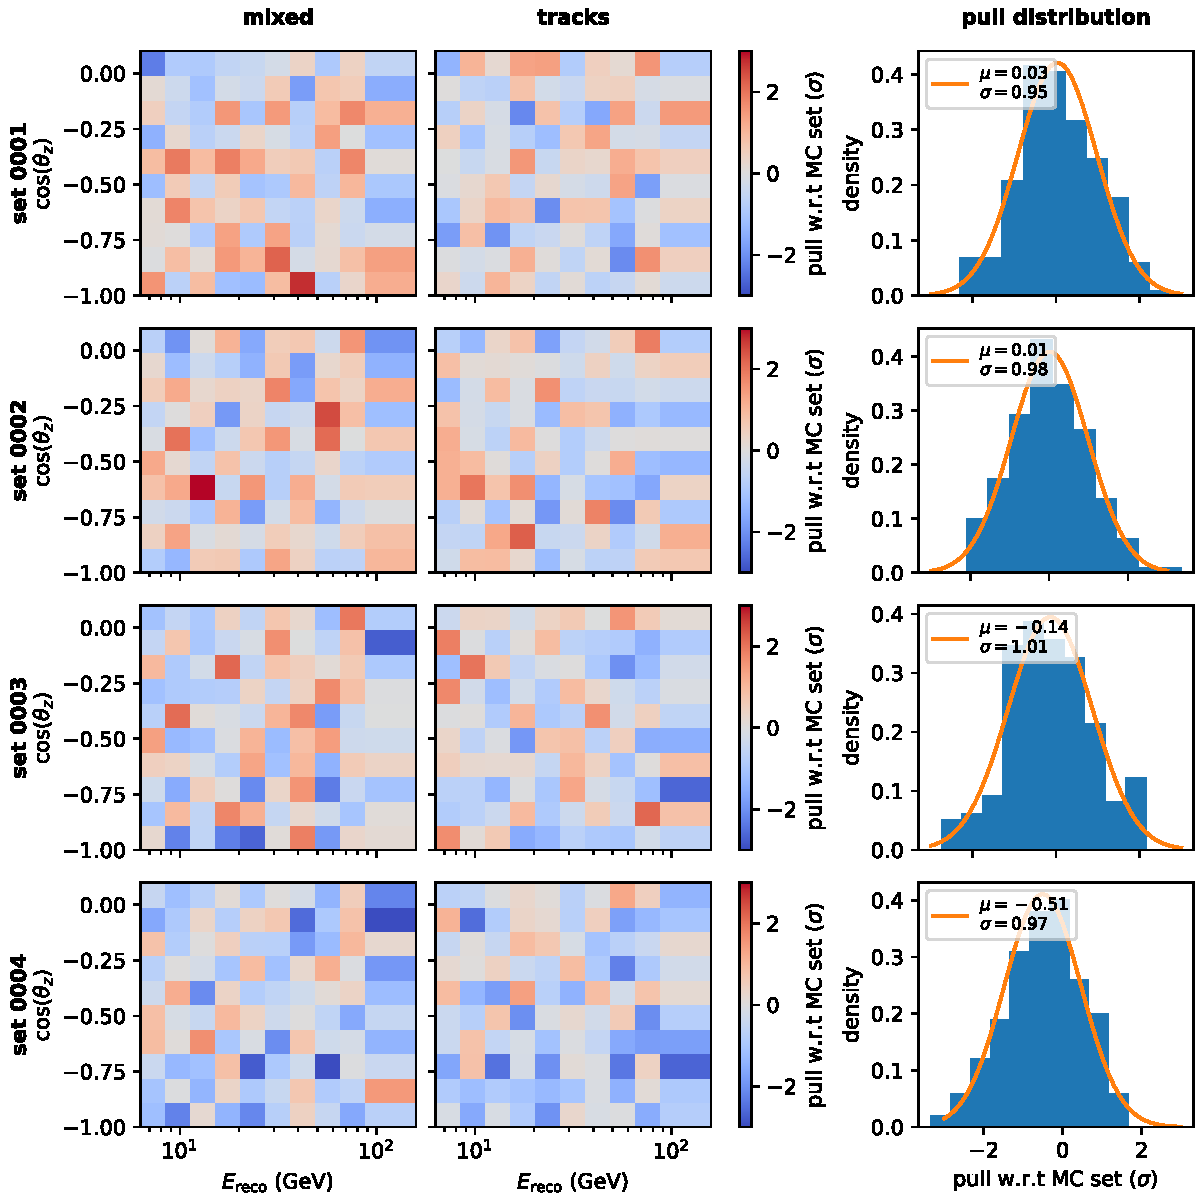
\includegraphics[width=0.9\textwidth]{figures/measurement/systematics/detector/ultrasurface_performance_vs_blind_fits_domeff_sets.pdf}
    \caption{Binwise pulls between the nominal set after re-weighting according to eq.~\ref{eq:ultrasurf-eval} and the systematic MC sets 0001, 0002, 0003, and 0004 representing DOM efficiency values of 90\%, 95\%, 105\%, and 110\%, resepctively. The 1D histogram in each row shows the distribution of the pulls over all bins.}
    \label{fig:ultrasurf-binwise-pulls}
\end{figure}

\begin{figure*}
    \centering
    \begin{subfigure}{0.4\linewidth}
        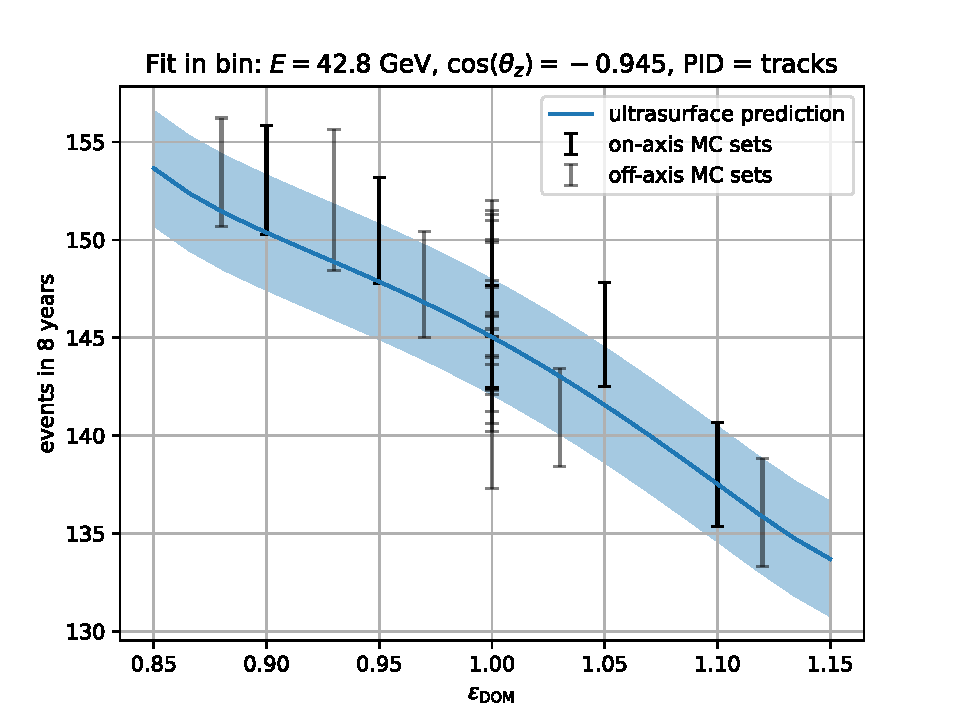
\includegraphics[width=\linewidth]{figures/measurement/systematics/detector/dom_eff_prediction.pdf}
        \caption{Prediction at best fit point of three-flavor analysis}
    \end{subfigure}
    %\hfill
    \begin{subfigure}{0.4\linewidth}
        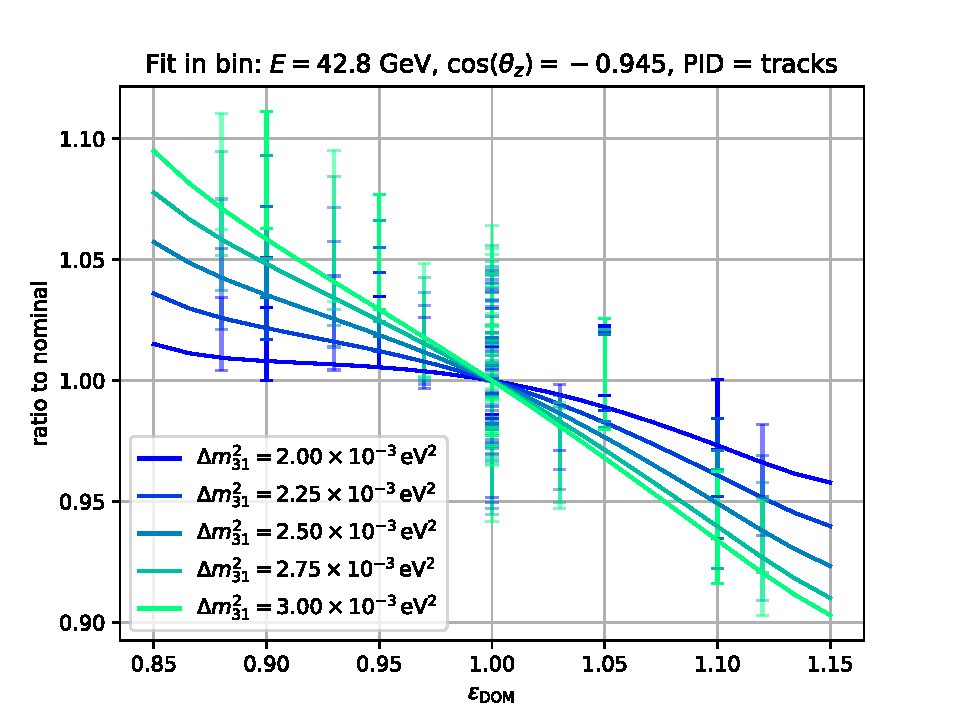
\includegraphics[width=\linewidth]{figures/measurement/systematics/detector/dom_eff_mass_splitting_scan.pdf}
        \caption{Prediction at different mass splitting values.}
    \end{subfigure}
    \caption{Prediction of bin counts in one bin of the analysis as a function of the DOM efficiency scale, $\epsilon_{\rm DOM}$. The error band in the left panel corresponds to the error on the nominal MC prediction without errors on the event-wise gradients.}
    \label{fig:dom-eff-prediction}
\end{figure*}



\subsection{Selection of Free Parameters}
\label{sec:sterile-analysis-parameter-selection}
To reduce the computational cost of optimizing the likelihood in a high-dimensional space, the impact of each nuisance parameter in consideration is assessed and its value fixed if it is found to be negligible.
Since the standard three-flavor oscillation model is a nested hypothesis within the 3+1 model, the parameter selection described in \refsec{std-osc-free-parameters} is taken as a starting point for the parameter selection of this analysis.
Starting from that selection, a test is run to determine if a paraemter is entirely dominated by its prior.
For this test, 200 trials are run where all nuisance parameters are sampled randomly according to their prior.
Then,  Asimov pseudo-data is produced at that point, and this pseudo-data is fit back with the default fit settings.
The resulting pairs of true injected parameter values and fitted values for every free parameter are shown in a scatter plot in \reffig{parameter-ensemble-result}.
If a parameter is entirely dominated by its prior, it will fit back to its nominal value regardless of the injected value.
For parameters where this is the case, their value is fixed to their nominal value during a fit.
Parameters to which this applies are framed in red in \reffig{parameter-ensemble-result}.
The framed parameters are (from top to bottom and from left to right in the bottom row): \texttt{barr\_w\_K}, \texttt{barr\_w\_antiK}, \texttt{barr\_g\_Pi}, \texttt{pion\_ratio}, \texttt{barr\_h\_Pi}.
The test shown in the figure was run before the priors on \texttt{barr\_i\_Pi}, \texttt{barr\_z\_K}, and \texttt{barr\_z\_antiK} have been inflated as described in \refsec{flux_systs}.
After that change,  \texttt{barr\_i\_Pi} was also added to the set of free parameters of the analysis.
The full list of free parameters with their respective ranges and priors is shown in \reftab{all-parameters}.

\begin{figure*}
    \centering
    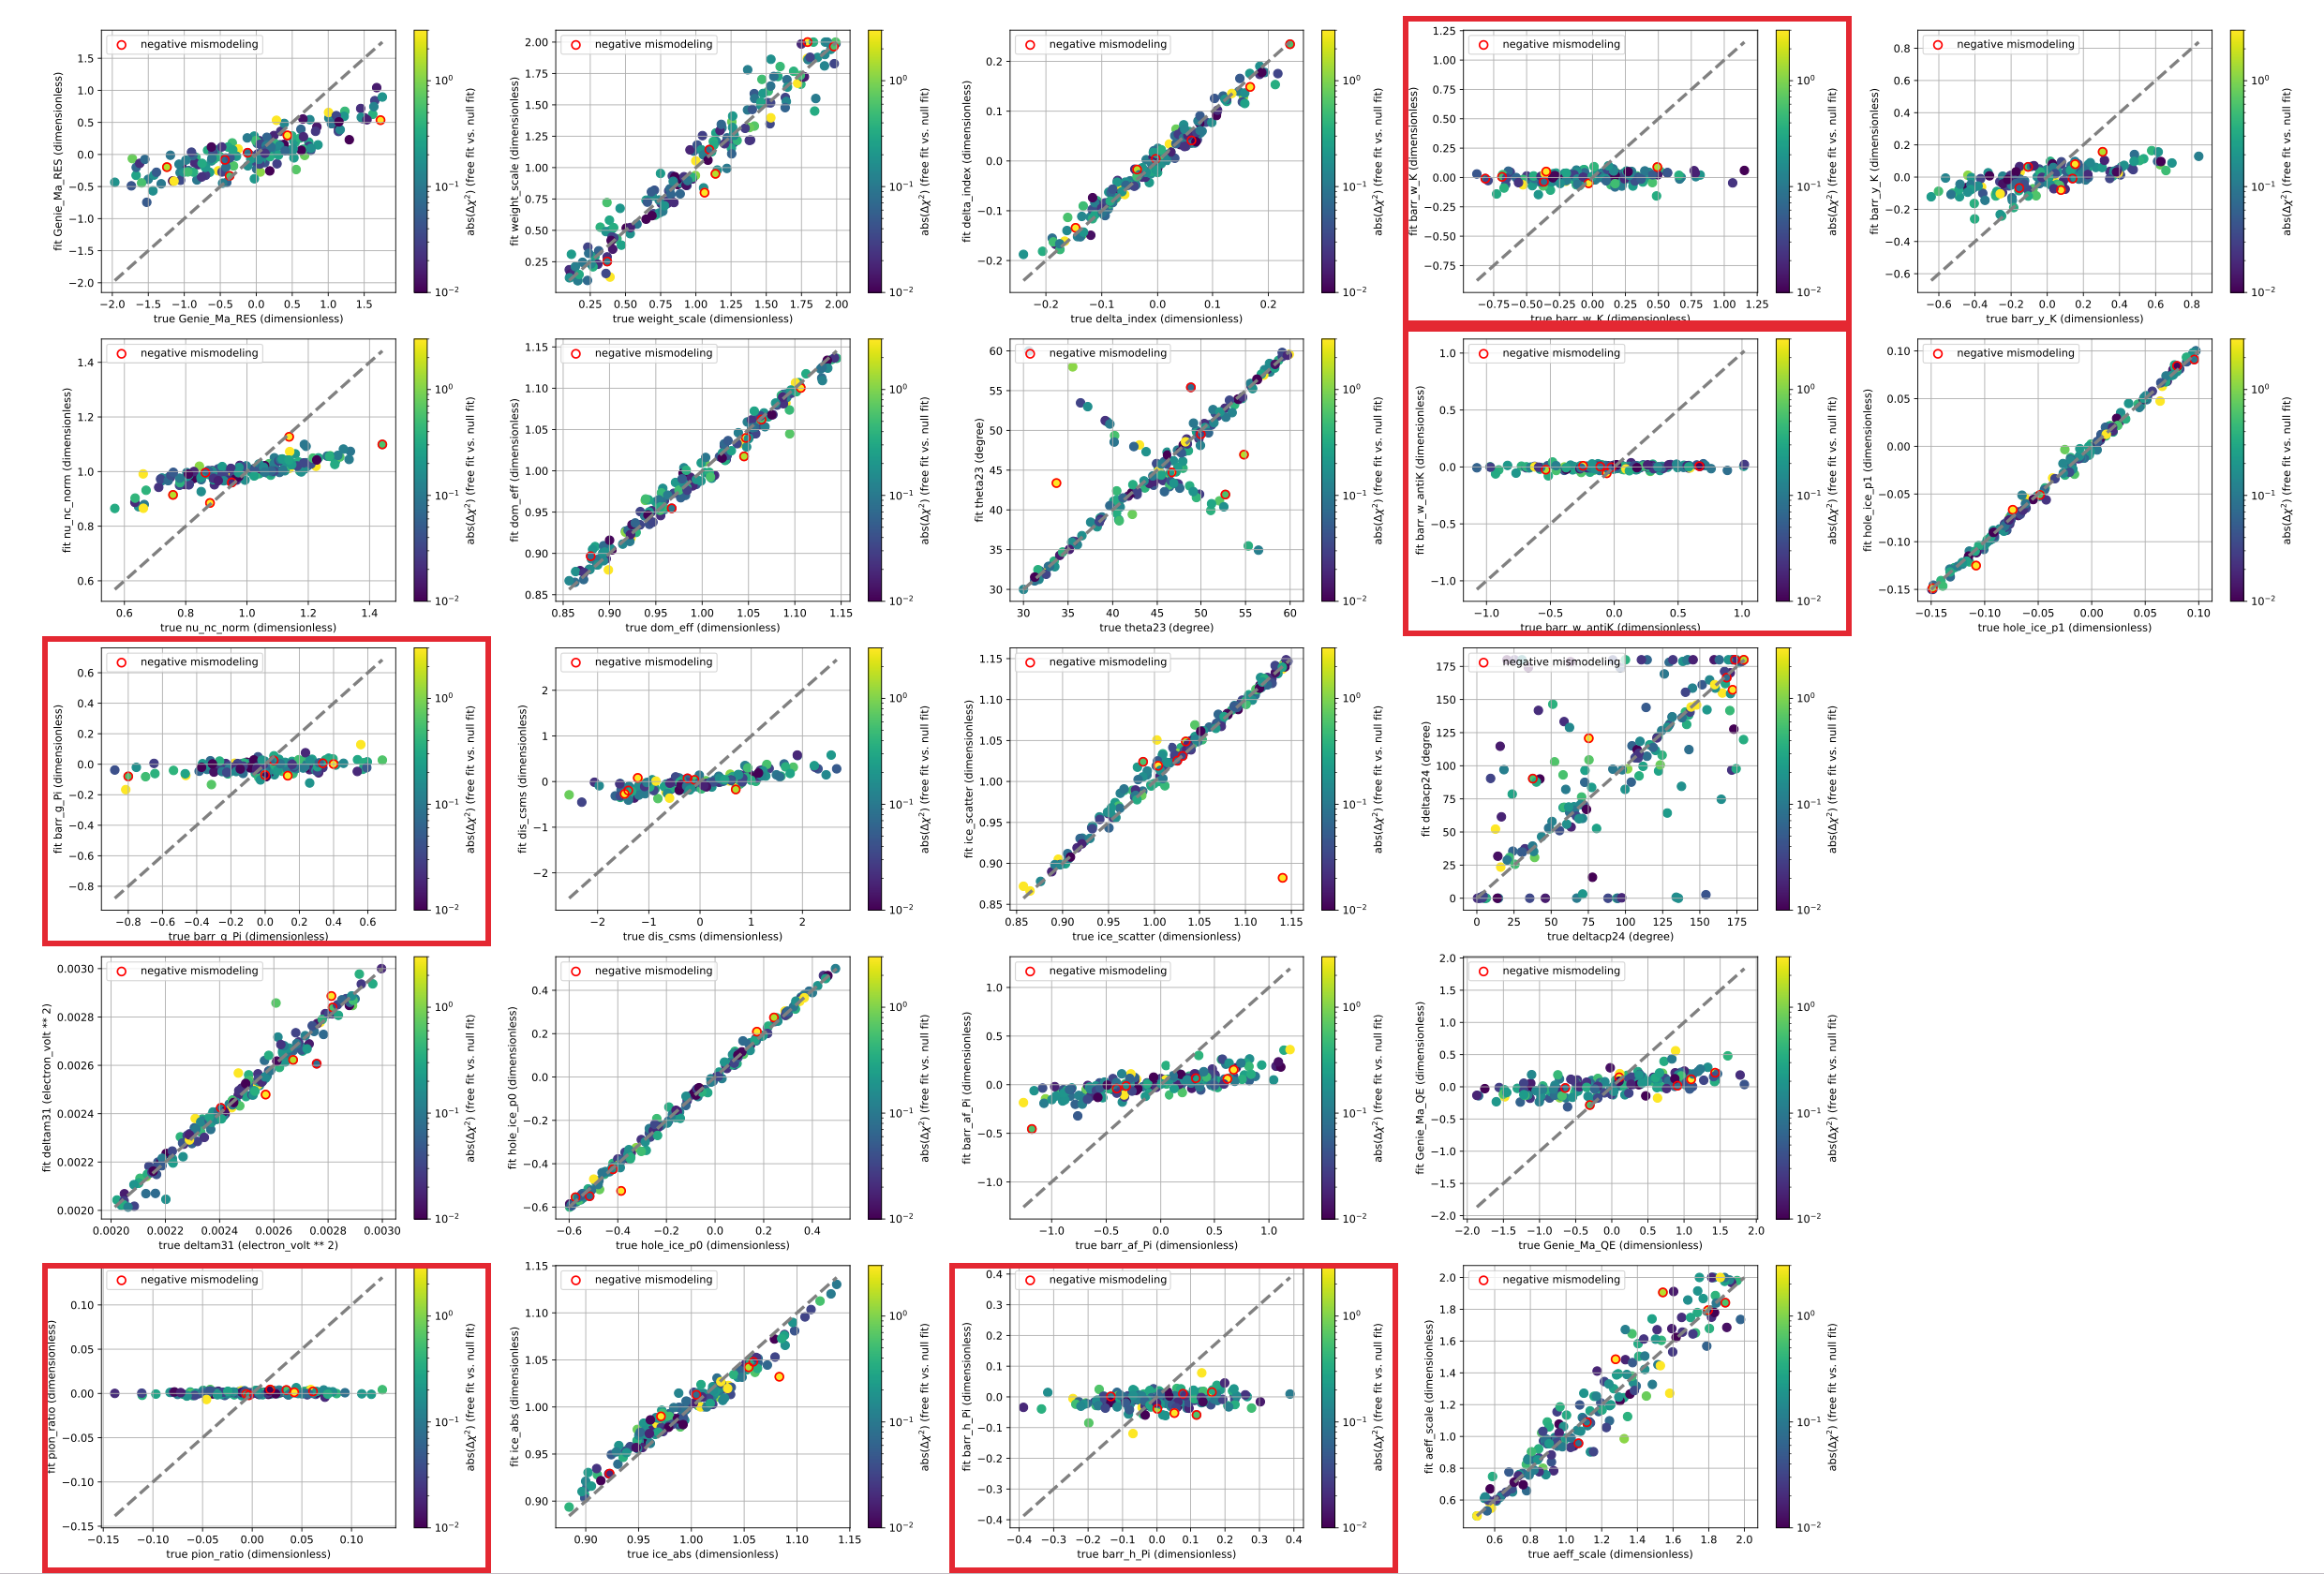
\includegraphics{figures/measurement/sterile_analysis/param_selection/Screen Shot 2022-05-30 at 13.12.49.png}
    \caption{Result of the ensemble test with randomly injected nuisance parameters. This test was run before the priors on \texttt{barr\_i\_Pi}, \texttt{barr\_z\_K}, and \texttt{barr\_z\_antiK} have been inflated as described in \refsec{flux_systs}. Parameters framed in red have been deemed to be negligible for the analysis. The color scale shows the likelihood difference between the free fit and a fit in which the physics parameters ($\theta_{24}$, $\theta_{34}$ have been fixed to their true value. If this number is negative, the trial is circled in red. In such cases, the minimizer failed to find the correct global optimum in the free fit.}
    \label{fig:parameter-ensemble-result}
\end{figure*}

\begin{table}
    \centering
    \begin{tabular}{cccl}\toprule
        \textbf{parameter} & \textbf{nominal value} & \textbf{range} & \textbf{prior} \\
        \midrule
        $\theta_{24}$ &    $0^\circ$ &  $0^\circ$ to $45^\circ$  & uniform \\
        $\theta_{34}$ &    $0^\circ$ &  $0^\circ$ to $45^\circ$  & uniform \\
        $\theta_{23}$ & $49.6^\circ$ & $20^\circ$ to $70^\circ$  & uniform \\
        $\delta_{24}$ &    $0^\circ$ &  $0^\circ$ to $180^\circ$ & uniform \\
        $\Delta m^2_{31}$ & $2.525\times10^{-3}\;\mathrm{eV^2}$ & $(2\,\rm{to}\, 3)\times10^{-3}\;\mathrm{eV^2}$ & uniform \\
        \midrule
        $\Delta \gamma_\nu$ & 0.0 & $-3\sigma$ to $+3\sigma$ &  $\sigma=0.1$  \\
        $\rm{Barr}, \: a-f_{\pi^+}$ & 0.0 & $-3\sigma$ to $+3\sigma$ &  $\sigma=0.63$  \\
        $\rm{Barr}, \: i_{\pi^+}$ & 0.0 & $-3\sigma$ to $+3\sigma$ &  $\sigma=0.61$  \\
        $\rm{Barr}, \: y_{K^+}$ & 0.0 & $-3\sigma$ to $+3\sigma$ &  $\sigma=0.3$  \\
        \midrule
        $M_{A,QE}$ & 0.0 & $-2\sigma$ to $+2\sigma$ &  $\sigma=1.0$  \\
        $M_{A,res}$ & 0.0 & $-2\sigma$ to $+2\sigma$ &  $\sigma=1.0$  \\
        DIS & 0.0 & $-3\sigma$ to $+3\sigma$ &  $\sigma=1.0$  \\
        $N_{\nu, NC}$ & 1.0 & 0.5 to 1.5 &  $\sigma=0.2$  \\
        \midrule
        $N_{\nu}$ & 1.0 & 0.5 to 2.0 & uniform \\
        $N_{\mu}$ & 1.0 & 0 to 3 & uniform \\
        \midrule
        $\epsilon_{\rm{DOM}}$ & 1.0 & 0.85 to 1.15 & $\sigma=0.1$ \\
        $\rm{ice \; absorption}$ & 1.0 & 0.85 to 1.15 & $\sigma=0.05$ \\
        $\rm{ice \; scattering}$ & 1.05 & 0.85 to 1.15 & $\sigma=0.1$ \\
        $\rm{hole \; ice}, \: p_0$ & 0.101569 & -1.1 to 0.5 & uniform \\
        $\rm{hole \; ice}, \: p_1$ & -0.049344 & -0.15 to 0.1 & uniform \\
        \bottomrule
    \end{tabular}
    \caption{List of all free parameters in the sterile oscillation analysis with their respective ranges and priors (if applicable).}
    \label{tab:all-parameters}
\end{table}

\subsection{Likelihood Optimization}
The optimization of the likelihood of the sterile oscillation model is considerably more difficult than that of the standard three-flavor oscillation analysis due to the increased complexity of the parameter interactions.
Two additional approximate degeneracies arise in the likelihood space from the sterile mixing angles alone: Firstly, for every best-fit point in $|U_{\mu 4}|$ and $|U_{\tau 4}|$, there will also be another local optimum where $|U_{\mu 4}|$ and $|U_{\tau 4}|$ are flipped\todo{Add example likelihood scan demonstrating this effect}.
In what follows, this is termed the \emph{triangle} degeneracy.
Secondly, flipping the sign of $\cos(\delta_{24})$, that is, flipping the \emph{quadrant} of $\delta_{24}$ around the angle of $90^\circ$, usually also results in another local minimum.
Together with the octant degeneracy of $\theta_{23}$, this means that at least eight local minima have to be checked for every fit.
During the development of this analysis, it was found that the likelihood is not entirely convex even within each of these eight distinct segments, leading to a poor performance of local second-order optimizers such as \textsc{migrad}\cite{minuit-algo}.
For this reason, the search for the global optimum in this analysis is done in three steps that are run separately for every combination of triangle, quadrant and octant.
The first step is a global optimization within each segment of the parameter space using the CRS2\cite{crs2} algorithm with a population of 300 samples.
The optimum found by CRS2 is then taken as the starting point for a local, derivative-free optimization using the \textsc{SbPlx}\cite{subplex} algorithm from the \textsc{nlopt}\cite{nlopt} package.
Finally, the best fit point from  \textsc{SbPlx} is used as a starting point to ''polish'' the result using \textsc{migrad}\cite{minuit-algo}.

\subsection{Analysis Checks}

The sterile oscillation analysis follows a procedure similar to that of the three-flavor oscillation analysis, in which the true results for nuisance and physics parameters are only revealed after a good fit quality has been established.
Because the data sample used to run the analysis is exactly the same, the checks for post-fit agreement between data and simulation and the seasonal stability need not be repeated.
However, the increased complexity of the likelihood space due to the increased number of oscillation parameters requires additional tests to ensure that the true optimum has been reached.

% \subsubsection{Low-pass filtering}
% As described in \refsec{low-pass-filtering}, the performance of the oscillation calculation is greatly improved by applying low-pass filters when evaluating the vacuum part of the Hamiltonian.

\subsubsection{Fit Convergence}

The inject/recover test with randomly sampled physics and nuisance parameters described in \refsec{sterile-analysis-parameter-selection} is used to quantify the reliability with which the correct global optimum is found.
To do this, a second fit is run for each trial where the values of $\theta_{24}$ and $\theta_{34}$ are fixed to their true values.
If the test statistic for this fit is smaller than that of the free fit, then the global optimization is proven to have failed to find the correct optimum.
Trials for which this is the case are marked in \reffig{parameter-ensemble-result} with red circles as having negative mis-modeling values.
It is apparent from \reffig{parameter-ensemble-result} that this is the case for a small percentage of trials.
The failure rate decreases after the parameters framed in red are fixed.
With the final parameter selection and minimization scheme, the rate of minimization failure found in this test is X\%\todo{Find fraction of failed fits for final selection}.
Because it is not possible to generally prove the success of a fit, the failure rate of this test can only provide a lower bound to the true failure rate.
The failure rate of the optimization could be reduced by either splitting the likelihood space into even more chunks, or by increasing the number of samples used by the \textsc{CRS2} search, but only at a significant increase to the already considerable computational cost of the analysis.
For the real data fit, the convergence of the likelihood is ensured by running a second fit where the physics parameters are fixed to the best fit point of the free fit.
The best fit parameter values and the test statistic of both fits are compared with a script that only prints the differences between them without revealing their absolute values to the analyzer, and the results will only be revealed if they are close to within minimizer precision.

\subsubsection{Goodness of Fit}
In a similar fashion as for the three-flavor oscillation analysis, the goodness of fit is established using an ensemble of pseudo-data trials with fluctuations taking both the MC uncertainty and the Poisson fluctuation of the data into account.
The pseudo-data expectation is generated by injecting the best fit values of the real data fit as true values.
The distribution of test statistic values resulting from this ensemble compared to that of the real data fit is shown in \reffig{sterile-modchi2-ensemble-comparison}.
The p-value of the observed test statistic is 22.5\%, demonstrating that the goodness of fit is well within the expectation.

\begin{figure}
    \centering
    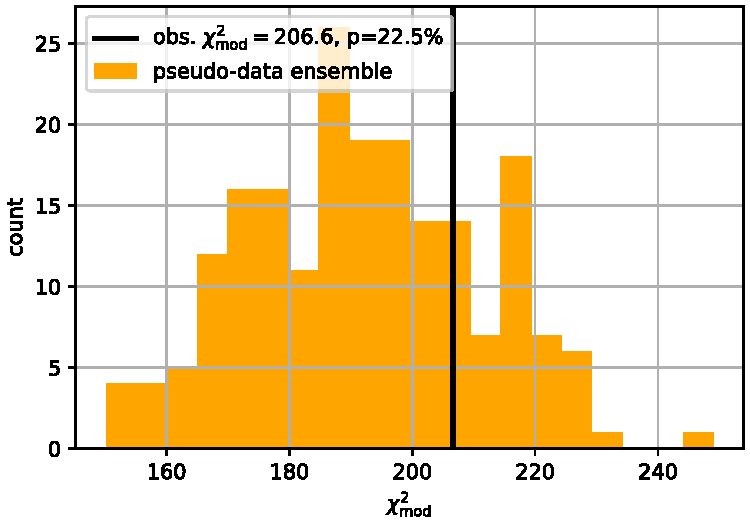
\includegraphics[width=0.8\linewidth]{figures/measurement/sterile_analysis/results/compare_ts_to_ensemble_REAL_DATA_FIT_v12_ext_holeice.pdf}
    \caption{Observed test statistic compared to the distribution expected from pseudo-data trials for the sterile oscillation analysis.}
    \label{fig:sterile-modchi2-ensemble-comparison}
\end{figure}

\section{Results}

\subsection{Best Fit Parameters}
The best fit result\todo{calculate errors} for the mixing amplitudes is
\begin{align*}
    |U_{\mu 4}|^2  &= 0.00449 \\
    |U_{\tau 4}|^2 &= 0.00307\;.
\end{align*}
Such small mixing amplitudes lie very well below the sensitivity of the analysis and are practically indistinguishable from the null hypothesis, in which there is no sterile neutrino mixing.
The value of the sterile CP-violating phase $\delta_{24}$ is inconsequential at such low sterile mixing amplitudes.
The best fit values of the nuisance parameters are shown in \reftab{nuisance_params_fittedval_sterile}.
Both analyses prefer close to maximal mixing in the atmospheric mixing angle $\theta_{23}$ and the atmospheric mass splitting fits to a value in the sterile oscillation fit that is only slightly higher than that of the three-flavor fit.
Almost all of the remaining nuisance parameters fit into their respective $1\sigma$ intervals, except for the scattering coefficient of the bulk ice, which pulls down by $1.5\sigma$ of its prior to a value of close to 90\%.
A comparison to the corresponding best fit parameters of the three-flavor oscillation analysis in \reftab{nuisance_params_fittedval} shows that most variables are in agreement in their general trend, but that the magnitude of their deviations from the baseline point is on average larger in the sterile oscillation analysis.
For instance, both fits prefer a harder cosmic ray spectrum, a higher DOM efficiency and less forward angular acceptance than nominal (see \reffig{hole-ice-bfp-comparison}), but the effect is more pronounced in the sterile oscillation fit in each case.
The best fit point of the sterile analysis also prefers an even higher atmospheric muon background than the three-flavor fit.

The oscillation parameters themselves are unlikely to explain these differences, since the sterile oscillation analysis fits very close to the null hypothesis of no sterile mixing.
However, there are two major distinctions in the implementation of both analyses in addition to the oscillation model that might be responsible for the observed discrepancies.
First, the weighting scheme that implements the effect of systematic uncertainties of detector properties is fundamentally different between both analyses.
In the three-flavor analyses, bin-wise linear regressions provided a prediction of the expected bin count for a given set of detector parameters as described in \refsec{hypersurfaces}.
These predictions reduce the statistical uncertainty by incorporating the information from all the MC sets, but depend on the particular choice of parameters at which the linear regressions were performed.
In the sterile analysis, each individual MC event is re-weighted using gradients that are fully decoupled from the choice of flux and oscillation parameters that are derived in \refsec{ultrasurfaces}.
The downside of this method is that the statistical uncertainty of the MC prediction is increased.
It is possible that the coupling of the detector response to the flux and oscillation parameters in the three-flavor fit and the increased statistical uncertainty in the sterile oscillation fit contribute to the different fit outcomes.
The second major difference between the fits is the choice of free parameters, in particular with respect to the parameterization of the meson production in the atmosphere with ''Barr blocks'' described in \refsec{barr-scheme}.
The sterile analysis allows only a small number of meson production parameters to be varied, but includes the high-energy pion fluctuation in the $I$ block (see \reffig{barr-blocks}) to vary with an increased prior width.
\todo{Inquire if more work should be done to find out what exactly is to blame.} To determine the precise degree to which the implementation details are responsible for the different fit outcomes is beyond the scope of this work.

\begin{table}
    \centering
    \caption{Fitted values of all nuisance parameters from the all-season sterile oscillation fit. The pull of the best fit value is shown for parameters with a defined prior.}
    \label{tab:nuisance_params_fittedval_sterile}
    \begin{tabular}{clSS} \toprule
        category & Parameter  & {Best Fit Value} &  {Pull ($\sigma$)} \\ \midrule
        \multirow{7}{5em}{$\nu$ flux}& $\Delta \gamma_\nu$ & 0.091 & 0.91 \\
        & Barr $\pi_\mathrm{AF}$ & 0.106  &  0.169 \\
        & Barr $\pi_\mathrm{I}$ & 0.446  &  0.731 \\
        & Barr $K_\mathrm{Y}$ & -0.0401  &  -0.134 \\ \midrule
        \multirow{4}{5em}{cross-section}& $M_{A}^{CCQE}$ &  -0.05  &  -0.050 \\
        & $M_{A}^{CCRES}$ & 0.0947  &  0.095  \\
        & DIS CSMS & 0.301  &  0.301 \\
        & NC norm & 1.005 &  0.024 \\ \midrule
        \multirow{5}{5em}{detector systematics} & $\epsilon_\mathrm{DOM}$ & 1.08  &  0.812 \\
        & hole ice $p_0$ & -0.589  &  \\
        & hole ice $p_1$ & 0.0408  &  \\
        & ice absorption & 0.988  &  -0.243\\
        & ice scattering & 0.895  &  -1.546\\ \midrule
        \multirow{3}{5em}{oscillation} & $\Delta m^{2}_{32}$ & \SI{2.476e-3}{\electronvolt\squared} & \\
        & $\sin^{2}\theta_{23}$ & 0.502 & \\
        & $\delta_{24}$ & \ang{180} & \\ \midrule
        \multirow{2}{5em}{norm}& $N_\mu$ & 1.93  &  \\
        & $N_\nu$ & 0.744 &  \\
        \bottomrule
    \end{tabular}
\end{table}

\subsection{Likelihood Scan and Contour}
The likelihood is scanned over $|U_{\mu 4}|$ and $|U_{\tau 4}|$ while marginalizing over all other parameters, including the standard three-flavor oscillation parameters and $\delta_{24}$.
The degeneracies in $\theta_{23}$ and $\delta_{24}$ are broken by running four separate fits, one for each possible combination of octant and quadrant.
An additional local \textsc{migrad} optimization is run for every grid point of the scan, in which all nuisance parameters start from the global best-fit point.
The test statistic value used in the scan is the optimum out of these five fits.
The test statistic values on the entire grid and the 90\% and 99\% C.L.
contours assuming Wilks' theorem with two degrees of freedom are shown in \reffig{sterile-contour-scan}.
For both $|U_{\mu 4}|$ and $|U_{\tau 4}|$, the analysis can constrain the amplitude of active-sterile mixing to $<0.1$ at $>99\%$ C.L., setting the strongest limit on $|U_{\tau 4}|$ to date.

The assumption that Wilks' theorem holds is certainly violated in some parts of the parameter space, especially in regions of very small sterile mixing due to boundary effects and the fact that the CP-violating phase $\delta_{24}$ can no longer provide a degree of freedom if either mixing amplitude is zero.
The coverage of the assumed $\chi^2$ distribution is tested on three points along the contour to determine if it is over-covering or under-covering using an ensemble of 200 pseudo-data trials, where the point to be tested is injected as the truth.
The right panel of \reffig{sterile-contour-scan} shows the distribution of the test statistic for each of the points that were tested together with the 90\% quantile from the ensemble and the expectation from Wilks' Theorem.
In each case, the 90\% quantile of the trials lies below the expected value, suggesting that the likelihood is over-covering and that the contour is therefore conservative.
As expected, this effect is stronger when one of the mixing amplitudes is close to zero.

% \begin{figure}
%     \centering
%     %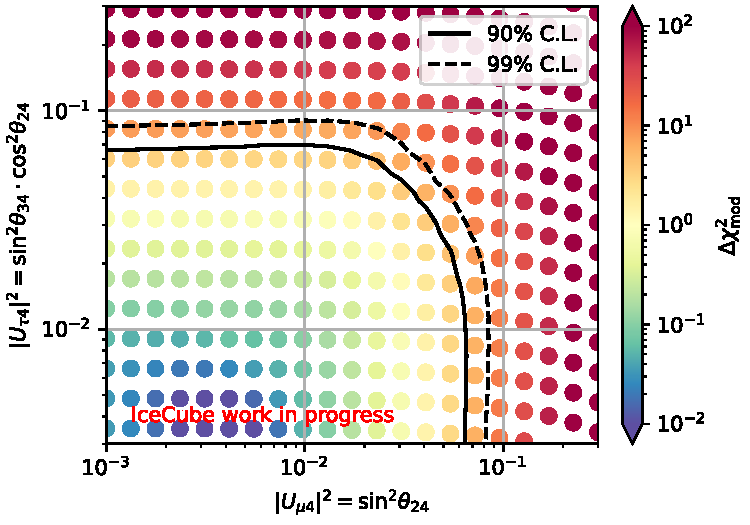
\includegraphics{figures/measurement/sterile_analysis/results/REAL_DATA_wilks_contours_merged_scans.pdf}
%     \tikzsetnextfilename{sterile_metric_scan}%
\begin{tikzpicture}

% Define new pgfmath function for the logarithm to base 10 that also works with fpu library
\pgfmathdeclarefunction{lg10}{1}{%
    \pgfmathparse{ln(#1)/ln(10)}%
}

\tikzstyle{bfp}=[very thick, orange, shape=diamond, fill=white, fill opacity=0.8, scale=0.8]


\begin{loglogaxis}[
	%view={0}{90},
	%enlargelimits,
    width=6.5cm,
    height=6.5cm,
    %height=0.9\linewidth,
    colorbar,
    colorbar style={
        %ytick={-2, -1, 0, 1, 2},
        yticklabel={$10^{\pgfmathprintnumber{\tick}}$},
        ylabel=$\Delta \chi^2_{\mathrm{mod}}$,
        tick align=outside,
        tick pos=right,
        tick style={color=black}
    },
    colorbar/width=0.4 cm,
    colormap/viridis,
    point meta min=-2.2,
    point meta max=2.2,
    clip marker paths=true,
    legend columns=2,
    xmin=8e-4, xmax=0.2,
    ymin=8e-4, ymax=0.5,
    ylabel={$|U_{\tau 4}|^2 = \sin^2\theta_{34}\cos^2\theta_{24}$},
    xlabel={$|U_{\mu 4}|^2 = \sin^2\theta_{24}$},
    xmajorgrids, ymajorgrids,
    tick align=outside,
    tick pos=left,
    tick style={color=black}
]
    \addplot [
        scatter,
        only marks,
        scatter src=explicit,
        mark size=3,
        forget plot
    ] table [
    	col sep=comma,
        x=Umu4_sq,
        y=Utau4_sq,
        %meta=metric_diff
        meta expr=lg10(\thisrow{metric_diff})
    ] {figures/measurement/sterile_analysis/results/contour_data/real_data_v12_metric_diff.csv};
	
    \addplot [black, very thick] table [col sep=comma,x=Umu4_sq,y=Utau4_sq] {figures/measurement/sterile_analysis/results/contour_data/real_data_v12_wilks_contour_90pct.csv};
    \addlegendentry{90\% C.L.}
    \addplot [black, very thick, dashed] table [col sep=comma,x=Umu4_sq,y=Utau4_sq] {figures/measurement/sterile_analysis/results/contour_data/real_data_v12_wilks_contour_99pct.csv};
    \addlegendentry{99\% C.L.}

    \addplot [scatter, only marks, mark=*, black] coordinates {
        (0.063, 0.001)
        (0.023, 0.059)
        (0.001, 0.066)
    };
    \addlegendentry{test points}

\node[draw, bfp] at (0.004578826816037697, 0.0029866619869177565) {};
\addlegendimage{legend image code/.code={
	\node[draw, bfp, scale=0.8] at (0cm,0cm) {};
    }
}
\addlegendentry{best fit point}

% One could also use TeX to plot the contours directly from the likelihood as below, but that 
% requires LuaLaTeX.

% level68: 2.27886856637673, lg10 = 0.357719278
% level90: 4.605170185988092, lg10 = 0.6632456844
% level99: 9.21034037197618, lg10 = 0.96427568
% level5sig: 28.743702426548186, lg10 = 1.4585427081

%	\addplot3 [
%        contour lua={
%        	%levels={4.605170185988092, 9.21034037197618, 28.743702426548186}
%			levels={0.6632456844, 0.96427568, 1.4585427081}
%		},
%		thick,
%        mesh/ordering=y varies,
%        mesh/rows=20,
%        mesh/cols=21,
%        %point meta=42
%    ] table [
%    	col sep=comma,
%		x=Umu4_sq,
%		y=Utau4_sq,
%		z expr=lg10(\thisrow{metric_diff})
%	] {contours/real_data_v12_metric_diff.csv};
    
\end{loglogaxis}
\end{tikzpicture}

%     \caption{Scan of the $\chi^2_{\mathrm{mod}}$ difference with respect to the best fit point with 90\% and 99\% C.L. contours assuming Wilks' theorem with two degrees of freedom.}
%     \label{fig:sterile-contour-scan}
% \end{figure}

\begin{figure*}
    \centering
    %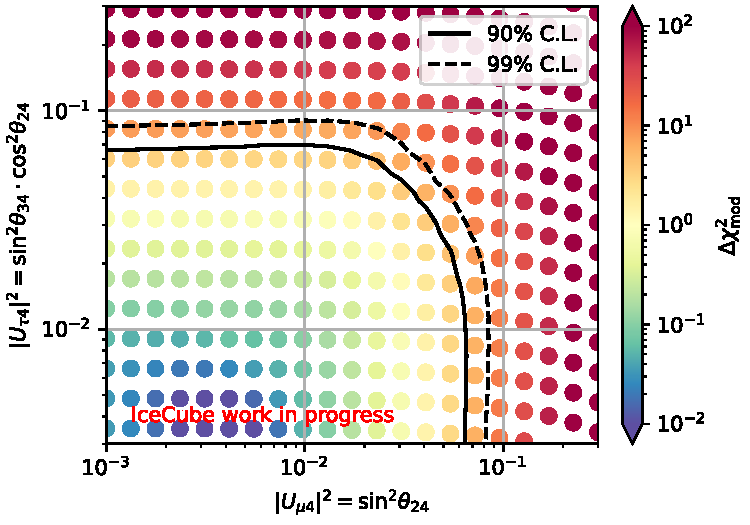
\includegraphics{figures/measurement/sterile_analysis/results/REAL_DATA_wilks_contours_merged_scans.pdf}
    \tikzsetnextfilename{sterile_metric_scan}%
\begin{tikzpicture}

% Define new pgfmath function for the logarithm to base 10 that also works with fpu library
\pgfmathdeclarefunction{lg10}{1}{%
    \pgfmathparse{ln(#1)/ln(10)}%
}

\tikzstyle{bfp}=[very thick, orange, shape=diamond, fill=white, fill opacity=0.8, scale=0.8]


\begin{loglogaxis}[
	%view={0}{90},
	%enlargelimits,
    width=6.5cm,
    height=6.5cm,
    %height=0.9\linewidth,
    colorbar,
    colorbar style={
        %ytick={-2, -1, 0, 1, 2},
        yticklabel={$10^{\pgfmathprintnumber{\tick}}$},
        ylabel=$\Delta \chi^2_{\mathrm{mod}}$,
        tick align=outside,
        tick pos=right,
        tick style={color=black}
    },
    colorbar/width=0.4 cm,
    colormap/viridis,
    point meta min=-2.2,
    point meta max=2.2,
    clip marker paths=true,
    legend columns=2,
    xmin=8e-4, xmax=0.2,
    ymin=8e-4, ymax=0.5,
    ylabel={$|U_{\tau 4}|^2 = \sin^2\theta_{34}\cos^2\theta_{24}$},
    xlabel={$|U_{\mu 4}|^2 = \sin^2\theta_{24}$},
    xmajorgrids, ymajorgrids,
    tick align=outside,
    tick pos=left,
    tick style={color=black}
]
    \addplot [
        scatter,
        only marks,
        scatter src=explicit,
        mark size=3,
        forget plot
    ] table [
    	col sep=comma,
        x=Umu4_sq,
        y=Utau4_sq,
        %meta=metric_diff
        meta expr=lg10(\thisrow{metric_diff})
    ] {figures/measurement/sterile_analysis/results/contour_data/real_data_v12_metric_diff.csv};
	
    \addplot [black, very thick] table [col sep=comma,x=Umu4_sq,y=Utau4_sq] {figures/measurement/sterile_analysis/results/contour_data/real_data_v12_wilks_contour_90pct.csv};
    \addlegendentry{90\% C.L.}
    \addplot [black, very thick, dashed] table [col sep=comma,x=Umu4_sq,y=Utau4_sq] {figures/measurement/sterile_analysis/results/contour_data/real_data_v12_wilks_contour_99pct.csv};
    \addlegendentry{99\% C.L.}

    \addplot [scatter, only marks, mark=*, black] coordinates {
        (0.063, 0.001)
        (0.023, 0.059)
        (0.001, 0.066)
    };
    \addlegendentry{test points}

\node[draw, bfp] at (0.004578826816037697, 0.0029866619869177565) {};
\addlegendimage{legend image code/.code={
	\node[draw, bfp, scale=0.8] at (0cm,0cm) {};
    }
}
\addlegendentry{best fit point}

% One could also use TeX to plot the contours directly from the likelihood as below, but that 
% requires LuaLaTeX.

% level68: 2.27886856637673, lg10 = 0.357719278
% level90: 4.605170185988092, lg10 = 0.6632456844
% level99: 9.21034037197618, lg10 = 0.96427568
% level5sig: 28.743702426548186, lg10 = 1.4585427081

%	\addplot3 [
%        contour lua={
%        	%levels={4.605170185988092, 9.21034037197618, 28.743702426548186}
%			levels={0.6632456844, 0.96427568, 1.4585427081}
%		},
%		thick,
%        mesh/ordering=y varies,
%        mesh/rows=20,
%        mesh/cols=21,
%        %point meta=42
%    ] table [
%    	col sep=comma,
%		x=Umu4_sq,
%		y=Utau4_sq,
%		z expr=lg10(\thisrow{metric_diff})
%	] {contours/real_data_v12_metric_diff.csv};
    
\end{loglogaxis}
\end{tikzpicture}

    \hfill
    \tikzsetnextfilename{fc_spot_checks}%
\begin{tikzpicture}


% level68: 2.27886856637673, lg10 = 0.357719278
% level90: 4.605170185988092, lg10 = 0.6632456844
% level99: 9.21034037197618, lg10 = 0.96427568
% level5sig: 28.743702426548186, lg10 = 1.4585427081

\begin{groupplot}[
    xmin=0, xmax=8,
    ymin=0, ymax=70,
    height=3 cm,
    width=6.5 cm,
    tick align=outside,
    tick pos=left,
    tick style={color=black},
    ylabel=count,
    legend columns=-1,
    group/.cd,
    columns=1,
    rows=3,
    vertical sep=10pt,
    xticklabels at=edge bottom
]

\nextgroupplot[
    legend style={at={(0.5, 1.0)}, anchor=south}
]
    \addplot [hist={data=x, bins=15}, fill=orange!75, draw=orange!50!black, ybar interval legend]
        file {figures/measurement/sterile_analysis/results/coverage_tests/coverage_test_stat_th24_14.4933015_th34_1.81215375.csv};
    \addlegendentry{ensemble}
    \addplot[black, thick, dashed] coordinates {
        (4.6, \pgfkeysvalueof{/pgfplots/ymin})
        (4.6, \pgfkeysvalueof{/pgfplots/ymax})
    };
    \node[anchor=south, font=\footnotesize\sffamily, rotate=90] at (4.6, 40) {4.6};
    \addlegendentry{Wilks' 90\%}
    \addplot[black, thick] coordinates {
        (2.99113419736533, \pgfkeysvalueof{/pgfplots/ymin})
        (2.99113419736533, \pgfkeysvalueof{/pgfplots/ymax})
    };
    \node[anchor=south, font=\footnotesize\sffamily, rotate=90] at (2.99113419736533, 40) {2.99};
    \addlegendentry{ensemble 90\%}

    \node[text width=1.8 cm, anchor=north east, font=\footnotesize] at (axis description cs:0.98, 0.98) {\begin{align*}|U_{\mu 4}|^2&=0.063 \\ |U_{\tau 4}|^2&=0.001\end{align*}};

\nextgroupplot
    \addplot [hist={data=x, bins=15}, fill=orange!75, draw=orange!50!black, ybar interval legend]
        file {figures/measurement/sterile_analysis/results/coverage_tests/coverage_test_stat_th24_8.78792305_th34_14.21562532.csv};
    %\addlegendentry{pseudo-data ensemble}
    \addplot[black, thick, dashed] coordinates {
        (4.6, \pgfkeysvalueof{/pgfplots/ymin})
        (4.6, \pgfkeysvalueof{/pgfplots/ymax})
    };
    \node[anchor=south, font=\footnotesize\sffamily, rotate=90] at (4.6, 40) {4.6};
    %\addlegendentry{Wilks' 90\% limit}
    \addplot[black, thick] coordinates {
        (3.5330841609355192, \pgfkeysvalueof{/pgfplots/ymin})
        (3.5330841609355192, \pgfkeysvalueof{/pgfplots/ymax})
    };
    \node[anchor=south, font=\footnotesize\sffamily, rotate=90] at (3.5330841609355192, 40) {3.53};
    %\addlegendentry{empirical 90\%}

    \node[text width=1.8 cm, anchor=north east, font=\footnotesize] at (axis description cs:0.98, 0.98) {\begin{align*}|U_{\mu 4}|^2&=0.023 \\ |U_{\tau 4}|^2&=0.059\end{align*}};

\nextgroupplot[xlabel={$\Delta \chi^2_\mathrm{mod}$}]
    \addplot [hist={data=x, bins=15}, fill=orange!75, draw=orange!50!black, ybar interval legend]
        file {figures/measurement/sterile_analysis/results/coverage_tests/coverage_test_stat_th24_1.81215375_th34_14.91525143.csv};
    %\addlegendentry{pseudo-data ensemble}
    \addplot[black, thick, dashed] coordinates {
        (4.6, \pgfkeysvalueof{/pgfplots/ymin})
        (4.6, \pgfkeysvalueof{/pgfplots/ymax})
    };
    \node[anchor=south, font=\footnotesize\sffamily, rotate=90] at (4.6, 40) {4.6};
    %\addlegendentry{Wilks' 90\% limit}
    \addplot[black, thick] coordinates {
        (2.423802342834482, \pgfkeysvalueof{/pgfplots/ymin})
        (2.423802342834482, \pgfkeysvalueof{/pgfplots/ymax})
    };
    \node[anchor=south, font=\footnotesize\sffamily, rotate=90] at (2.42, 40) {2.42};
    %\addlegendentry{empirical 90\%}

    \node[text width=1.8 cm, anchor=north east, font=\footnotesize] at (axis description cs:0.98, 0.98) {\begin{align*}|U_{\mu 4}|^2&=0.001 \\ |U_{\tau 4}|^2&=0.066\end{align*}};


\end{groupplot}

\end{tikzpicture}
    \caption{Scan of the $\chi^2_{\mathrm{mod}}$ difference with respect to the best fit point with 90\% and 99\% C.L. contours assuming Wilks' theorem with two degrees of freedom (left) and ensemble test of the coverage on three points along the 90\% C.L. line (right). The test points indicated in the left panel correspond to the points at which the ensemble test were produced in the right panel.}
    \label{fig:sterile-contour-scan}
\end{figure*}

\begin{figure*}
    \centering

    \tikzsetnextfilename{sterile_wilks_contour_context}%
\begin{tikzpicture}

\begin{loglogaxis}[
    width=0.45\linewidth,
    height=0.4\linewidth,
    xmin=1e-3, xmax=0.5,
    ymin=3e-3, ymax=7,
    xmajorgrids, ymajorgrids,
    y filter/.expression={y < 1e-3 ? ln(1e-3) : ln(y)},
    x filter/.expression={x < 1e-3 ? ln(1e-3) : ln(x)},
    legend columns=2,
    transpose legend=false,
    legend style={at={(0.98, 0.98)}, anchor=north east},
    ylabel={$|U_{\tau 4}|^2 = \sin^2\theta_{34}\cos^2\theta_{24}$},
    xlabel={$|U_{\mu 4}|^2 = \sin^2\theta_{24}$},
    tick align=outside,
    tick pos=left,
    tick style={color=black}
]

\addplot [orange, thick] table [col sep=comma] {figures/measurement/sterile_analysis/results/contour_data/ANTARES_90pct_free_dcp24.csv};
\addplot [orange, thick, forget plot] table [col sep=comma] {figures/measurement/sterile_analysis/results/contour_data/ANTARES_90pct_free_dcp24_2.csv};
\addlegendentry{ANT (2019)}


\addplot [orange, thick, dashed] table [col sep=comma] {figures/measurement/sterile_analysis/results/contour_data/ANTARES_90pct_fixed_dcp24.csv};
\addlegendentry{ANT (2019)}

\addplot [bluishgreen, thick, dashed] table [col sep=comma] {figures/measurement/sterile_analysis/results/contour_data/SK_90_pct.csv};
\addlegendentry{SK (2015)}

% MEOWS contours are given in sin^2(2theta_24), sin^2(2theta_34) and need to be converted
% to |Umu4|^2, |Utau4|^2 via
% 	|Umu4|^2 = sin(0.5 arcsin(sqrt(sin2_2theta24)))^2
% 	|Utau4|^2 = sin(0.5 arcsin(sqrt(sin2_2theta34)))^2 * cos(0.5 arcsin(sqrt(sin2_2theta24)))^2
\addplot [vermilion, thick, dashed] table [
	col sep=comma,
	x expr=sin(0.5 * asin(sqrt(\thisrowno{0})))^2,
	y expr=sin(0.5 * asin(sqrt(\thisrowno{1})))^2 * cos(0.5 * asin(sqrt(\thisrowno{0})))^2,
] {figures/measurement/sterile_analysis/results/contour_data/meows_mixing_90pct.csv};
\addlegendentry{IC (2020)}


% NOvA's contours are flipped!!!
\addplot [skyblue, thick, dashed] table [
	x index=1,
	y index=0,
	col sep=comma
] {figures/measurement/sterile_analysis/results/contour_data/nova_90pct_matrix_elems.csv};
\addlegendentry{NO$\nu$A (2017)}

\addplot [black, very thick] table [col sep=comma,x=Umu4_sq,y=Utau4_sq] {figures/measurement/sterile_analysis/results/contour_data/real_data_v12_wilks_contour_90pct.csv};
\addlegendentry{this work}


\node[plot annotation, text width=3.5 cm, anchor=south west] at (axis description cs:0.01, 0.01) {All contours 90\% C.L., \par dashed lines imply $\delta_{24}=0$};
\node[font=\sffamily\footnotesize, red, anchor=north east] at (axis description cs:0.95, 0.7) {\emph{IceCube preliminary}};

\end{loglogaxis}

\end{tikzpicture}

    \tikzsetnextfilename{sterile_wilks_contour_leesard}%
\begin{tikzpicture}

\begin{loglogaxis}[
    width=0.45\linewidth,
    height=0.4\linewidth,
    xmin=1e-3, xmax=0.5,
    ymin=3e-3, ymax=7,
    xmajorgrids, ymajorgrids,
    y filter/.expression={y < 1e-3 ? ln(1e-3) : ln(y)},
    x filter/.expression={x < 1e-3 ? ln(1e-3) : ln(x)},
    legend columns=1,
    legend style={at={(0.98, 0.98)}, anchor=north east},
    transpose legend=false,
    ylabel={$|U_{\tau 4}|^2 = \sin^2\theta_{34}\cos^2\theta_{24}$},
    xlabel={$|U_{\mu 4}|^2 = \sin^2\theta_{24}$},
    tick align=outside,
    tick pos=left,
    tick style={color=black}
]

\addplot [blue, thick] table [col sep=comma] {figures/measurement/sterile_analysis/results/contour_data/IceCube_90_IO.csv};
\addlegendentry{IC (2017), IO}

\addplot [orange, thick] table [col sep=comma] {figures/measurement/sterile_analysis/results/contour_data/IceCube_90_pct.csv};
\addlegendentry{IC (2017), NO}


\addplot [black, very thick] table [col sep=comma,x=Umu4_sq,y=Utau4_sq] {figures/measurement/sterile_analysis/results/contour_data/real_data_v12_wilks_contour_90pct.csv};
\addlegendentry{this work}


\node[plot annotation, anchor=south west] at (axis description cs:0.01, 0.01) {All contours 90\% C.L.};
\node[font=\sffamily\footnotesize, red, anchor=north east] at (axis description cs:0.95, 0.7) {\emph{IceCube preliminary}};

\end{loglogaxis}

\end{tikzpicture}

    \caption{Contour of the 90\% C.L. of this analysis compared to measurements from the ANTARES\cite{ANTARES:2018rtf}, Super-Kamiokande\cite{Super-Kamiokande:2014ndf} and NO$\nu$A\cite{nova-sterile} experiments and a previous high-energy IceCube oscillation study\cite{MEOWS} (left), and compared to the previous DeepCore study\cite{deepcore_sterile_2017} (right).}
    \label{fig:sterile-contour-context}
\end{figure*}

% \begin{figure}
%     \centering
%     \tikzsetnextfilename{sterile_wilks_contour_leesard}%
\begin{tikzpicture}

\begin{loglogaxis}[
    width=0.45\linewidth,
    height=0.4\linewidth,
    xmin=1e-3, xmax=0.5,
    ymin=3e-3, ymax=7,
    xmajorgrids, ymajorgrids,
    y filter/.expression={y < 1e-3 ? ln(1e-3) : ln(y)},
    x filter/.expression={x < 1e-3 ? ln(1e-3) : ln(x)},
    legend columns=1,
    legend style={at={(0.98, 0.98)}, anchor=north east},
    transpose legend=false,
    ylabel={$|U_{\tau 4}|^2 = \sin^2\theta_{34}\cos^2\theta_{24}$},
    xlabel={$|U_{\mu 4}|^2 = \sin^2\theta_{24}$},
    tick align=outside,
    tick pos=left,
    tick style={color=black}
]

\addplot [blue, thick] table [col sep=comma] {figures/measurement/sterile_analysis/results/contour_data/IceCube_90_IO.csv};
\addlegendentry{IC (2017), IO}

\addplot [orange, thick] table [col sep=comma] {figures/measurement/sterile_analysis/results/contour_data/IceCube_90_pct.csv};
\addlegendentry{IC (2017), NO}


\addplot [black, very thick] table [col sep=comma,x=Umu4_sq,y=Utau4_sq] {figures/measurement/sterile_analysis/results/contour_data/real_data_v12_wilks_contour_90pct.csv};
\addlegendentry{this work}


\node[plot annotation, anchor=south west] at (axis description cs:0.01, 0.01) {All contours 90\% C.L.};
\node[font=\sffamily\footnotesize, red, anchor=north east] at (axis description cs:0.95, 0.7) {\emph{IceCube preliminary}};

\end{loglogaxis}

\end{tikzpicture}

%     \caption{Contour of the 90\% C.L. of this analysis compared to the previous DeepCore study\cite{deepcore_sterile_2017}.}
%     \label{fig:sterile-contour-leesard}
% \end{figure}
